\documentclass[12pt,a4paper]{article}

% Basic Packages
\usepackage[utf8]{inputenc}
\usepackage[T1]{fontenc}
\usepackage{geometry}
\usepackage{graphicx}
\usepackage{microtype}
\usepackage{subfiles}
\usepackage{enumitem}
\usepackage{lipsum}
\usepackage{tikz-cd}
\usepackage{pifont}  % For Pifont symbols
\usepackage{tikz}
\usepackage{titlesec}
\usepackage{appendix}

% Mathematics Packages
\usepackage{amsmath, amssymb, amsthm}
\usepackage{mathtools}
\numberwithin{equation}{section}

% For improved tables
\usepackage{booktabs}

% For improved referencing
\usepackage{hyperref}

% Custom theorem environments
\newtheorem{theorem}{Theorem}[section]
\newtheorem{lemma}[theorem]{Lemma}
\newtheorem{corollary}[theorem]{Corollary}
\newtheorem{proposition}[theorem]{Proposition}
\newtheorem{definition}[theorem]{Definition}
\newtheorem{remark}[theorem]{Remark}
\newtheorem{example}[theorem]{Example}
\newtheorem{claim}[theorem]{Claim}

\renewcommand\epsilon{\ensuremath{\varepsilon}}

% Page geometry (adjust margins as needed)
\geometry{
  left=25mm,
  right=25mm,
  top=25mm,
  bottom=25mm
}

% Title, author, and date
\title{Lie Algebra (Co)Homology}
\date{\today} % or specify a date manually

\begin{document}

\maketitle % Print the title
\tableofcontents

\section{Introduction} % (fold)
\label{sec:Introduction}
In this mini project we study reflective subcategories and their properties. To motivate this a little bit, consider the category of abelian groups which are contained in the category of groups. The abelianization functor then serves as a left adjoint to this inclusion. We can then consider the monad induced by this adjunction and ask ourselves if the category of $ T $-algebras on groups ($ T $ being the monad) is equivalent to the category of abelian groups. As we shall see, this is indeed the case, and it follows from the result that the inclusion of a reflective subcategory is monadic.

We\footnote{``We'' is used only as a literary device, as this is solely my own work.} have chosen to answer the questions that accompany this mini project as an extended text which we have tried to fit together in a logical manner. Section~\ref{sec:Preliminaries} answers questions 1--4 while section~\ref{sec:Monadic Structure of Reflective Subcategories} answers question 5. More specifically, we have the map between questions and theorems/propositions/lemmas as shown in Figure~\ref{fig:map}.
\begin{figure}[ht]
  \begin{center}
    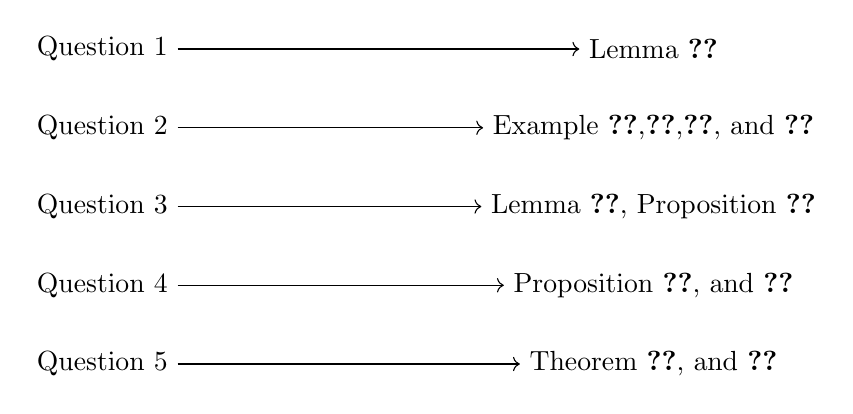
\begin{tikzpicture}
      \node (Q1) at (0,4) {Question 1};
      \node (Q2) at (0,3) {Question 2};
      \node (Q3) at (0,2) {Question 3};
      \node (Q4) at (0,1) {Question 4};
      \node (Q5) at (0,0) {Question 5};
      \node (A1) at (7,4) {Lemma~\ref{lem:adjprops}};
      \node (A2) at (7,3) {Example~\ref{ex:ab},\ref{ex:ring},\ref{ex:met}, and \ref{ex:haus}};
      \node (A3) at (7,2) {Lemma~\ref{lem:ess}, Proposition~\ref{prop:local}};
      \node (A4) at (7,1) {Proposition~\ref{prop:creates}, and~\ref{prop:colims}};
      \node (A5) at (7,0) {Theorem~\ref{thm:beck}, and~\ref{thm:converse}};
      \draw[->] (Q1) -- (A1);
      \draw[->] (Q2) -- (A2);
      \draw[->] (Q3) -- (A3);
      \draw[->] (Q4) -- (A4);
      \draw[->] (Q5) -- (A5);
      % Add more nodes and arrows as needed
    \end{tikzpicture}
  \end{center}
  \caption{Correspondence between questions in the mini project problem sheet and the appropriate results in this text.}\label{fig:map}
\end{figure}

% section Introduction (end)

\section{Lie Algebras and $ \mathfrak{g} $-modules} % (fold)
\label{sec:Lie Algebras}
\subsection{Basics of Lie Algebras} % (fold)
\label{sub:Basics of Lie Algebras}
We will assume throughout this project that $ k $ is a field.
\begin{definition}[Lie Algebra]
  A \textbf{Lie algebra} is a $ k $-module $ \mathfrak{g} $ equipped with a bilinear skew-symmetric map $ [-,-]: \mathfrak{g} \times \mathfrak{g} \to \mathfrak{g} $ which satisfies the Jacobi identity:
  \begin{equation}
    \forall x,y,z \in \mathfrak{g}\, [x,[y,z]] + [z, [x, y]] + [y, [z, x]] = 0
    \label{eq:jacobi}
  .\end{equation}
  A morphism of Lie algebras $ \phi: \mathfrak{g} \to \mathfrak{h} $ is a $ k $-linear map which respects the bracket, i.e.,
  \begin{equation}
    \phi([x,y]) = [\phi(x), \phi(y)].
    \label{eq:liehom}
  \end{equation}
\end{definition}

For any associative algebra $ A $ there is a natural Lie algebra $ \mathfrak{a}\coloneqq \text{Lie}(A) $ where, for $ x,y \in A $, one defines
\begin{equation*}
  [x,y] = xy - yx
.\end{equation*}
It is straightforward to verify that $ [-,-]: \mathfrak{a} \times \mathfrak{a} \to \mathfrak{a} $ satisfies the Jacobi identity.

\begin{lemma}
  \label{lem:functoriality}
  The assignment $ \text{Lie}:k\text{-}\mathbf{Alg} \to k\text{-}\mathbf{LieAlg} $ as defined above is a functor.
\end{lemma}
\begin{proof}
  Let $ f: A \to B $ be a morphism of $ k $-algebras. The map $ \text{Lie}(f):\text{Lie}(A) \to \text{Lie}(B) $ defined for $ x \in \text{Lie}(A) $ by $ (\text{Lie}(f))(x)=f(x) $ is a Lie algebra morphism. To see this, let $ x,y \in A $, then
  \begin{align*}
    (\text{Lie}(f))([x,y]) &= f([x,y]) \\
                           &= f(xy - yx) \\
                           &= f(xy) - f(yx) \\
                           &= f(x)f(y) - f(y)f(x) \\
                           &= [f(x), f(y)] \\
                           &= [(\text{Lie}(f))(x), (\text{Lie}(f))(y)]
  \end{align*}
  and hence $ \text{Lie}(f) $ is indeed a Lie algebra homomorphism. It trivially holds that $ \text{Lie}(1_A) = 1_{\text{Lie}(A)} $. Hence the only thing that remains to be checked is that composition is preserved. Let $ f \in \text{Hom}_{k\text{-}\mathbf{Alg}}(A,B) $, $ g \in \text{Hom}_{k\text{-}\mathbf{Alg}}(B,C) $. We then have that
  \begin{align*}
    \text{Lie}(g \circ f) &= g \circ f \\
                          &= \text{Lie}(g) \circ \text{Lie}(f)
  .\end{align*}
\end{proof}

It turns out that Lie has a left adjoint $ U: k\text{-}\mathbf{LieAlg} \to k\text{-}\mathbf{Alg} $ called the universal enveloping algebra. In order to define this functor we must first talk about tensor algebras.

\begin{definition}[Tensor algebra]
  If $ M $ is any $ k $-module, then the \textbf{tensor algebra} $ T(M) $ is the graded associative $ k $-algebra with unit generated by $ M $:
  \begin{equation}
    T(M) \coloneqq \bigoplus_{n = 0}^{\infty} M^{\otimes n}
    \label{eq:gaa}
  \end{equation}
  where $ M^{\otimes n} = \bigotimes_{i = 1}^{n} M $ for $ n>0 $ and $ M^{\otimes 0}=k $. Multiplication is defined by concatenation of terms in the obvious way.
\end{definition}

It is straightforward to verify that $ T $ defines a functor from the category of $ k $-modules to the category of associative unital $ k $-algebras. Using $ T $ we can the proceed to define the universal enveloping algebra of a Lie algebra $ \mathfrak{g} $:

\begin{definition}[Universal enveloping algebra]
  If $ \mathfrak{g} \in k\text{-}\mathbf{LieAlg} $, then the \textbf{universal enveloping algebra} $ U\mathfrak{g} $ is the quotient of $ T\mathfrak{g} $ by the two sided ideal $ I_\mathfrak{g} $ generated by the relations
  \begin{equation}
    i(x) \otimes i(y) - i(y) \otimes i(x) - i([x,y]),\quad (x,y \in \mathfrak{g}).
    \label{eq:relations}
  \end{equation}
  where $ i: \mathfrak{g} \to T\mathfrak{g} $ is the inclusion map.
\end{definition}

The relations in Equation~\ref{eq:relations} makes $ i:\mathfrak{g} \to \text{Lie}(U\mathfrak{g}) $ into a Lie algebra homomorphism. Technically $ i $ is the inclusion $ i: \mathfrak{g} \to T\mathfrak{g} $ followed by the projection $ p: T\mathfrak{g} \to U\mathfrak{g} $ but we will denote it by $ i $ nonetheless (this is justified as we shall see).


Let $ \{e_{\alpha}\} $ be a fixed and ordered basis for some Lie algebra $ \mathfrak{g} $ over $ k $.
If $ I = (\alpha_1, \ldots, \alpha_p) $ is a sequence of indices we will abuse notation to let $ e_I $ denote the image of $ e_{\alpha_1} \otimes \cdots \otimes e_{\alpha_p} $ in $ U\mathfrak{g} $. The sequence $ I $ is called \textbf{increasing} if $ \alpha_1 \leq \ldots \leq \alpha_p $. The empty sequence $ \phi = () $ is also regarded as increasing and we set $ e_\phi = 1 $. Note that if $ I = (\alpha) $ is a single index then $ e_\alpha \in \mathfrak{g} $ while $ e_{(\alpha)} \in U\mathfrak{g} $.

\begin{theorem}[Poincar\'e-Birkhoff-Witt Theorem]
  \label{thm:pbw}
  If $ \mathfrak{g} $ is a free $ k $-module, then $ U\mathfrak{g} $ is also a free $ k $-module. If $ \{e_{\alpha}\} $ is an ordered basis of $ \mathfrak{g} $, then the elements $ e_I $ with $ I $ an increasing sequence form a basis of $ U\mathfrak{g} $.
\end{theorem}
\begin{proof}
  See \cite[V.2]{jacobson1979lie}.
\end{proof}

Note that since we assume $ k $ is a field it follows that every $ k $-module is free and hence the Poincar\'e-Birkhoff-Witt theorem will always apply for us.

\begin{corollary}
  The map $ i: \mathfrak{g} \to U\mathfrak{g} $ as defined earlier is an injection identifying $ \mathfrak{g} $ with $ i(\mathfrak{g}) $. Moreover $ U\mathfrak{g} $ is the free $ k $-algebra generated by $ i(\mathfrak{g}) $.
\end{corollary}
\begin{proof}
  As each basis element of $ \mathfrak{g} $ is mapped to a basis element of $ U\mathfrak{g} $ the first part follows from the Poincar\'e-Birkhoff-Witt theorem. The second part also follows from the Poincar\'e-Birkhoff-Witt theorem: if $ \{e_{\alpha}\} $ is an ordered basis for $ \mathfrak{g} $ then $ i(e_\alpha) = e_{(\alpha)} $ and since $ e_{(\alpha)}e_{(\beta)} = e_{(\alpha, \beta)} $ it follows that all basis elements of $ U\mathfrak{g} $ can be generated from the multiplication of elements of the form $ e_{(\alpha)} $. As we define the multiplication of zero elements to be the unit $ 1 \in k $ we have that $ i(\mathfrak{g}) $ does indeed generate $ U\mathfrak{g} $ as a free $ k $-algebra.
\end{proof}

Later we will be interested in creating a projective resolution of $ U\mathfrak{g} $-modules and a good place to start is by defining a $ k $-algebra homomorphism $ U\mathfrak{g} \to k $.
\begin{definition}[Augmentation ideal]
  Let $ \{e_{\alpha}\} $ be an ordered basis for $ \mathfrak{g} $. The \textbf{augmentation ideal} of $ \mathfrak{g} $ is defined to be the kernel of the $ k $-algebra homomorphism $ \epsilon: U\mathfrak{g} \to k $ where $ \epsilon(e_{(\alpha)}) = 0 $ for all $ \alpha $. We denote this ideal by $ \mathfrak{J} = \text{ker}(\epsilon) $.
\end{definition}
It is fairly straightforward to see that $ k \cong U\mathfrak{g}/\mathfrak{J} $ as the only things which survive the quotienting process is the $ k $ in the 0th degree of $ U\mathfrak{g} $.

More can be said about the functor $ U $:
\begin{lemma}
  \label{lem:ufunct}
  The construction $ U:k\text{-}\mathbf{LieAlg} \to k\text{-}\mathbf{Alg} $ is functorial.
\end{lemma}
\begin{proof}
  We first note that for $ f \in \text{Hom}_{k\text{-}\mathbf{LieAlg}}(\mathfrak{g}, \mathfrak{h}) $, $ Uf: U\mathfrak{g} \to U\mathfrak{h} $ and $ x_1, \ldots, x_n \in \mathfrak{g} $ we have that
  \begin{equation}
    Uf(x_1\cdots x_n) = f(x_1)\cdots f(x_n)
    \label{eq:uf}
  \end{equation}
  where we abuse notation and let $ x_1\cdots x_n $ denote the equivalence class of $ x_1 \otimes \cdots \otimes x_n $ in $ U\mathfrak{g} $.
  This is well defined as for $ x,y \in \mathfrak{g} $ we have
  \begin{equation*}
    f(x \otimes y - y \otimes x - [x,y]) = f(x) \otimes f(y) - f(y) \otimes f(x) - [f(x), f(y)] \in I_{\mathfrak{h}}
  \end{equation*}
  where $ I_{\mathfrak{h}} $ denotes the two sided ideal used in the definition of $ U $. Hence $ Tf(I_\mathfrak{g}) \subset I_\mathfrak{h} $ and since $ Tf|_k = 1_k $ this descends to a morphism $ Uf:U\mathfrak{g} \to U\mathfrak{h} $.

  From Equation~\ref{eq:uf} it follows that
  \begin{equation*}
    U 1_{\mathfrak{g}} = 1_{U\mathfrak{g}}.
  \end{equation*}
  For $ x_1, \ldots, x_n \in \mathfrak{g} $, $ f \in \text{Hom}_{k\text{-}\mathbf{LieAlg}}(\mathfrak{g}, \mathfrak{h})  $, $  g \in \text{Hom}_{k\text{-}\mathbf{LieAlg}}(\mathfrak{h}, \mathfrak{l})  $ we have that
  \begin{align*}
    U(g \circ f)(x_1 \cdots x_n) &= g(f(x_1)) \cdots gf(x_n) \\
                                                     &= Ug(f(x_1) \cdots f(x_n)) \\
                                                     &= (Ug \circ Uf)(x_1 \cdots x_n)
  \end{align*}
  and hence
  \begin{equation}
    U(g \circ f) = Ug \circ Uf
  .\end{equation}
  We thus see that $ U:k\text{-}\mathbf{LieAlg} \to k\text{-}\mathbf{Alg} $ defines a functor.
\end{proof}

\begin{proposition}
  \label{prop:adjointu}
  The functor $  U:k\text{-}\mathbf{LieAlg} \to k\text{-}\mathbf{Alg}  $ is left adjoint to $ \text{Lie}:k\text{-}\mathbf{Alg} \to k\text{-}\mathbf{LieAlg} $.
\end{proposition}
\begin{proof}
  We do this by explicitly constructing the unit and counit. Define the unit $ \eta: 1_{k\text{-}\mathbf{LieAlg}} \implies \text{Lie}U $ componentwise by the inclusion map $ i_\mathfrak{g}: \mathfrak{g} \to \text{Lie}(U\mathfrak{g}) $
  i.e., $\eta_\mathfrak{g} = i_\mathfrak{g}$.
  We define the counit $ \epsilon: U\text{Lie} \implies 1_{k\text{-}\mathbf{Alg}} $ to be the evaluation map, i.e., for $ \{e_{\alpha}\} $ an ordered basis on $ \text{Lie}(A) $ and $ I = (\alpha_1, \ldots, \alpha_n) $ an increasing sequence we let
  \begin{equation}
    \epsilon_A(e_I) = (e_{\alpha_1}(\cdots (e_{\alpha_{n-1}}e_{\alpha_n})\cdots)).
  \end{equation}
  It is straightforward to verify that both $ \eta $ and $ \epsilon $ are natural constructions. To see this for $ \eta $ we let $ \phi:\mathfrak{g} \to \mathfrak{h} $ be a map between two $ k $-Lie algebras. We must then verify commutativity of the following diagram:
  \[\begin{tikzcd}
	  {\mathfrak{g}} & {\mathfrak{h}} \\
	  {\text{Lie}U\mathfrak{g}} & {\text{Lie}U\mathfrak{h}.}
	  \arrow["\phi", from=1-1, to=1-2]
	  \arrow["{\text{Lie}U\phi}"', from=2-1, to=2-2]
	  \arrow["{i_\mathfrak{g}}"', from=1-1, to=2-1]
	  \arrow["{i_\mathfrak{h}}", from=1-2, to=2-2]
  \end{tikzcd}\]
  It suffices to show commutativity on basis elements. Hence, let $ \{e_\alpha\} $ and $ \{d_\beta\} $ be ordered basis sets on $ \mathfrak{g} $ and $ \mathfrak{h} $ respectively. We then have that
  \begin{align*}
    i_\mathfrak{h}(\phi(e_\alpha)) &=i_\mathfrak{h}\left( \sum_{\beta} y_\beta d_\beta \right) \\
                                   &= \sum_{\beta} y_\beta d_{(\beta)} \\
                                   &= \text{Lie}U\phi \left( e_{(\alpha)} \right) \\
                                   &= \text{Lie}U\phi(i_\mathfrak{g}(e_\alpha))
  \end{align*}
  as desired. A similar argument works to show that $ \epsilon $ is natural.

  We must now verify the triangle identities:
  \begin{align*}
    \epsilon U \circ U\eta &= 1_U \\
    \text{Lie}\,\epsilon \circ \eta\,\text{Lie} &= 1_{\text{Lie}}.
  \end{align*}
  It suffices to verify it on basis elements. Let $ \{e_\alpha\} $ be an ordered basis on some $ k $-Lie algebra $ \mathfrak{g} $ and $ \{x_\beta\} $ an ordered basis on some associative $ k $-algebra $ A $ (both have basis as $ k $ is a field). Let $ I = (\alpha_1, \ldots, \alpha_n) $ be an increasing sequence. We then have
  \begin{align*}
    (\epsilon_{U\mathfrak{g}} \circ U\eta_\mathfrak{g})(e_I) &= \epsilon_{U\mathfrak{g}}(Ui_\mathfrak{g}(e_I)) \\
                                                             &= \epsilon_{U\mathfrak{g}}(\overline{e_I}) \\
                                                             &= e_I
  \end{align*}
  as desired, where $ \overline{e_I} $ is the equivalence class of $ e_I $ in $ U^2\mathfrak{g} $. Similarly, for $ x_\beta \in \{x_\beta\} $ we have
  \begin{align*}
    (\text{Lie}\,\epsilon_A \circ \eta_{\text{Lie}(A)})(x_\beta) &= \text{Lie}\,\epsilon_A (x_{(\beta)}) \\
                                                        &= x_\beta
  \end{align*}
  as desired. Hence $ \eta $ and $  \epsilon $ satisfy the requirement for $ U $ being left adjoint to $ \text{Lie} $.
\end{proof}


% subsection Basics of Lie Algebras (end)


\subsection{$\mathfrak{g}$-modules} % (fold)
\label{sub:g-modules}
Lie algebras are not rings and so the concept of $ \mathfrak{g} $-modules is not defined out of the box. However, there is a natural way in which a $ \mathfrak{g} $-module can make sense.
\begin{definition}[Left $ \mathfrak{g} $-module]
  Let $ \mathfrak{g} $ be a Lie algebra over the field $ k $. A \textbf{left} $ \mathfrak{g} $-\textbf{module} is a $ k $-module $ M $ together with a bilinear action map $ \mathfrak{g} \otimes_k M \to M $ such that $ x \otimes m $ maps to $ xm $ and
  \begin{equation}
    [x,y]m = x(ym) - y(xm).
    \label{eq:whoknow}
  \end{equation}
  Morphisms of left $ \mathfrak{g} $-modules $ M $ and $ N $ are $ k $-linear maps
  $ f: M \to N $ such that the following diagram commutes
  \[\begin{tikzcd}
	  {\mathfrak{g} \otimes_k M} & {\mathfrak{g} \otimes_k N} \\
	  M & N
	  \arrow[from=1-1, to=2-1]
	  \arrow["f"', from=2-1, to=2-2]
	  \arrow[from=1-2, to=2-2]
	  \arrow["{\text{1}_\mathfrak{g} \otimes f}", from=1-1, to=1-2]
  \end{tikzcd}\]
  where the vertical maps are the action maps.
\end{definition}

In order to use (co)homological methods on the category of $ \mathfrak{g} $-modules we need that it is abelian.
\begin{lemma}
  The category $ \mathfrak{g} $-\textbf{Mod} is preadditive.
\end{lemma}
\begin{proof}
  First, note that $ \text{Hom}_{\mathfrak{g}\text{-}\mathbf{Mod}}(M, N) $ is a subset of $ \text{Hom}_{k\text{-}\mathbf{Mod}}(M, N) $. In fact, it is a submodule since for $ \alpha \in k $ and $ f,g \in  \text{Hom}_{\mathfrak{g}\text{-}\mathbf{Mod}}(M, N) $ we have $ \alpha f \in  \text{Hom}_{\mathfrak{g}\text{-}\mathbf{Mod}}(M, N)  $ and $ f + g \in  \text{Hom}_{\mathfrak{g}\text{-}\mathbf{Mod}}(M, N)  $. Hence $  \text{Hom}_{\mathfrak{g}\text{-}\mathbf{Mod}}(M, N)  $ is a $ k $-submodule of $  \text{Hom}_{\mathfrak{k}\text{-}\mathbf{Mod}}(M, N)  $ and so is certainly abelian. That the composition $ \mathbb{Z} $-bilinear follows immediately since $  \text{Hom}_{\mathfrak{g}\text{-}\mathbf{Mod}}(M, N)  $ is a $ k $-submodule of $  \text{Hom}_{\mathfrak{k}\text{-}\mathbf{Mod}}(M, N)  $. Hence $ \mathfrak{g} $-\textbf{Mod} is preadditive.
\end{proof}

\begin{lemma}
  The category $ \mathfrak{g} $-\textbf{Mod} is additive.
\end{lemma}
\begin{proof}
  It is enough to show that $ \mathfrak{g} $-\textbf{Mod} has a zero object and binary coproducts. The zero object $ 0 \in k $-\textbf{Mod} works as a zero object in $ \mathfrak{g} $-\textbf{Mod} as well. We thus only need to show that it has binary coproducts.

  To this end, let $ M,N \in \mathfrak{g} $-\textbf{Mod}. Consider the direct sum of $ M $ and $ N $ as $ k $-modules $ M \oplus N $. We will give this a $ \mathfrak{g} $-module structure and show that satisfies the property of being the binary coproduct of $ M $ and $ N $ in the category of $ \mathfrak{g} $-modules. Note that $ \mathfrak{g} \otimes_k (M \oplus N) \cong (\mathfrak{g} \otimes_k M) \oplus (\mathfrak{g} \otimes_k N) $ as $ k $-modules. The two maps $ \mathfrak{g} \otimes_k M \to M $ and $ \mathfrak{g} \otimes_k N \to N $ then combine to give a map
  \begin{equation}
    \mathfrak{g} \otimes_k (M \oplus N) \cong (\mathfrak{g} \otimes_k M) \oplus (\mathfrak{g} \otimes_k N)  \to M \oplus N.
    \label{eq:bincop}
  \end{equation}
  For $ x,y \in \mathfrak{g} $ and $ m + n \in M \oplus N $ we then also have that
  \begin{align*}
    [x,y](m + n) &= [x,y]m + [x,y]n \\
                 &= x(ym) - y(xm) + x(yn) - y(xn) \\
                 &= x(y(m + n)) - y(x(m + n)),
  \end{align*}
  which is a necessary criteria for $ M \oplus N $ being given a $ \mathfrak{g} $-module structure. The inclusion maps $ M \to M \oplus N $ and $ N \to M \oplus N $ are then also $ \mathfrak{g} $-module morphisms.

  The only remaining thing to show then is that $ M \oplus N $ satisfies the universality property. Thus, let $ f: M \to P $ and $ g: N \to P $ be two $ \mathfrak{g} $-module morphisms. Viewing them as $ k $-module morphisms we know there is a $ k $-module morphism $ f \oplus g: M \oplus N \to P $. What remains to show is that it also a $ \mathfrak{g} $-module morphism. In other words, that the following diagram commutes
  \[\begin{tikzcd}
	  {\mathfrak{g} \otimes_k (M \oplus N)} & {\mathfrak{g} \otimes_k P} \\
	  {M\oplus N} & P
	  \arrow[from=1-1, to=2-1]
	  \arrow["{f\oplus g}"', from=2-1, to=2-2]
	  \arrow[from=1-2, to=2-2]
	  \arrow["{1_\mathfrak{g} \otimes (f \oplus g)}", from=1-1, to=1-2]
  \end{tikzcd}\]
  Pointwise we have that for $ m \in M $, $ n \in N $, and $ x \in \mathfrak{g} $
  \begin{align*}
    (f \oplus g) (x(m+n)) &= (f \oplus g)(xm + xn) \\
                          &= f(xm) + g(xn) \\
                          &= xf(m) + xg(n) \\
                          &= x(f(m) + g(n)) \\
                          &= x((f \oplus g)(m + n))
  \end{align*}
  and hence the diagram does indeed commute which means that $ f \oplus g $ is a $ \mathfrak{g} $-module morphism. Thus $ M \oplus N $ with the imposed $ \mathfrak{g} $-module structure satisfies the universality property and so $ \mathfrak{g} $-\textbf{Mod} has finite coproducts.
\end{proof}

\begin{lemma}
  The category $ \mathfrak{g} $-\textbf{Mod} is preabelian.
\end{lemma}
\begin{proof}
  This follows if we can show that for a given $ f \in \text{Hom}_{\mathfrak{g}\text{-}\mathbf{Mod}}(M ,N) $ the $ k $-modules $ \text{ker}(f) $ and $ \text{coker}(f) $ are also the kernel and cokernel, respectively, of $ f $.

  Suppose $ m \in \text{ker}(f) $ and $ x \in \mathfrak{g} $. Then $ f(xm) = xf(m) = 0 $ and hence $ \mathfrak{g} \otimes_k M \to M $ restricts to a map $ \mathfrak{g} \otimes_k \text{ker}(f) \to \text{ker}(f) $ which makes the following diagram commute:
  \[\begin{tikzcd}
	  {\mathfrak{g} \otimes_k \text{ker}(f)} & {\mathfrak{g} \otimes_k M} \\
	  {\text{ker}(f)} & M
	  \arrow[from=1-1, to=2-1]
	  \arrow["i"', from=2-1, to=2-2]
	  \arrow[from=1-2, to=2-2]
	  \arrow["{1_\mathfrak{g} \otimes i}", from=1-1, to=1-2]
  \end{tikzcd}\]
  Suppose next that there is a morphism $ g \in \text{Hom}_{\mathfrak{g}\text{-}\mathbf{Mod}}(P, M) $ such that $ g\circ f = 0 $. There is then a unique $ k $-module morphism $ \alpha:P \to \text{ker}(f) $ such that $ g = i\circ \alpha $. We just need to show that $ \alpha $ is also a $ \mathfrak{g} $-module morphism. Let $ x \in \mathfrak{g} $ and $ p \in P $, we then have
  \begin{align*}
    i(\alpha(xp)) &= g(xp) \\
                  &= xg(p) \\
                  &= x i(\alpha(p)) \\
                  &= i(x\alpha(p))
  \end{align*}
  and since $ i $ is injective we have $ \alpha(xp) = x\alpha(p) $ showing that $ \alpha $ is a $ \mathfrak{g} $-module morphism. Hence the universality of $ \text{ker}(f) $ has been established. That $ [x,y]m = x(ym) - y(xm) $ for $ m \in \text{ker}(f) $ follows immediately since $ \text{ker}(f) $ is a submodule of $ M $. Hence $ \text{ker}(f) $ is indeed the kernel of $ f $.

  Now, suppose $ n \in \text{im}(f) $ and $ x \in \mathfrak{g} $. Then $ n = f(m) $ for some $ m \in M $. Hence $ xn = xf(m) = f(xm) $ which means $ xn \in \text{im}(f) $ and so we have a commutative diagram
  \[\begin{tikzcd}
	  {\mathfrak{g} \otimes_k N} & {\mathfrak{g} \otimes_k \text{coker}(f)} \\
	  N & {\text{coker}(f)}
	  \arrow[from=1-1, to=2-1]
	  \arrow["\pi"', from=2-1, to=2-2]
	  \arrow["{1 \otimes \pi}", from=1-1, to=1-2]
	  \arrow[from=1-2, to=2-2]
  \end{tikzcd}\]
  where $ \pi $ is the projection. For $ \overline{n} \in \text{coker}(f) $ and $ x,y \in \mathfrak{g} $ the equality $ [x,y]\overline{n} = x(y\overline{n}) - y(x\overline{n}) $ follows directly from the commutativity of the above diagram. Hence, what remains is to check the universality condition. Let therefore $ g \in \text{Hom}_{\mathfrak{g}\text{-}\mathbf{Mod}}(N, P) $ such that $ g\circ f = 0 $. By the universality of $ \text{coker}(f) $, as a $ k $-module, there exists a unique $ k $-module map $ \alpha: P \to \text{coker}(f) $ such that $ g = \alpha \circ \pi $. We need to show that $ \alpha $ is a $ \mathfrak{g} $-module map as well. Hence let $ [n] \in \text{coker}(f) $ and $ x \in \mathfrak{g} $. We then have that
  \begin{align*}
    \alpha(x[n]) &= \alpha(x\pi(n)) \\
                 &= \alpha(\pi(xn)) \\
                 &= x\alpha(\pi(n)) \\
                 &= x\alpha([n])
  \end{align*}
  as desired.
\end{proof}

\begin{proposition}
  \label{prop:abelian}
  The category $ \mathfrak{g} $-\textbf{Mod} is abelian.
\end{proposition}
\begin{proof}
  What remains to show is that every monomorphism is the kernel of some morphism and every epimorphism is the cokernel of some morphism.

  Let therefore $ f \in \text{Hom}_{\mathfrak{g}\text{-}\mathbf{Mod}}(M, N) $ be a monomorphism. We then have that $ f $ is the kernel (considered as a $ k $-module) of $ \mathfrak{g} $-module morphism $ \pi: N \to \text{coker}(f) $. As $ k $-\textbf{Mod} is abelian, we have $ \text{ker}(\pi) = \text{im}(f) \cong M $. The proof of the previous lemma then gives the result.

  The same argumentation also works for epimorphisms. We therefore have that $ \mathfrak{g} $-\textbf{Mod} is abelian.
\end{proof}

More can be said about the structure of $ \mathfrak{g} $-\textbf{Mod}:
\begin{proposition}
  \label{prop:monoidal}
  The category $ \mathfrak{g} $-\textbf{Mod} is closed symmetric monoidal where the action map on $ M \otimes_k N $ is given by $ x(m \otimes n) = xm\otimes n + m\otimes xn $.
\end{proposition}
\begin{proof}
  See Appendix~\ref{sec:Closed Symmetric Monoidal Structure on}.
\end{proof}

Now, as $ \mathfrak{g} $-\textbf{Mod} is abelian, it makes sense to talk about projective and injective resolutions for objects $ M \in \mathfrak{g} $-\textbf{Mod}. We can then use these resolutions to talk about Ext and Tor which we use to define the (co)homology of $ M $.

In order to be able to do this we need that every $ \mathfrak{g} $-module has a projective and injective resolution.
\begin{lemma}
  \label{lem:eqcat}
  If $ F:\mathcal{A} \rightleftarrows \mathcal{B}: G $ is an equivalence of abelian categories then $ \mathcal{A} $ has enough projectives/injectives if and only if $ \mathcal{B} $ has enough projectives/injectives.
\end{lemma}
\begin{proof}
  Let $ F:\mathcal{A} \rightleftarrows \mathcal{B}:G $ be an equivalence of categories. Then $ F $ and $ G $ preserves projective/injective objects. Without loss of generality, assume that $ \mathcal{B} $ has enough projectives and let $ M \in \mathcal{A} $. We want to find a projective object $ P \in \mathcal{A} $ and an epimorphism $ \epsilon: P \to M $. Since $ \mathcal{B} $ has enough projectives we know that there exists a projective object $ P' \in \mathcal{B} $ and an epimorphism $ \epsilon': P' \to F(M) $. We then have that $ G(P') $ is projective in $ \mathcal{A} $ and $ G(\epsilon'):G(P') \to GF(M) $ is an epimorphism. We then use the isomorphism $ \eta_M^{-1}:GF(M) \cong M $ and define $ \epsilon = \eta_M^{-1} \circ \epsilon' $ which is still an epimorphism. Letting $ P = G(P') $ we have an epimorphism $ \epsilon: P \to M $ from a projective object $ P $ to $ M $ showing that $ \mathcal{A} $ has enough projectives.

  The other direction is proved similarly and the case for enough injectives follows by duality.
\end{proof}

\begin{lemma}
  \label{lem:ex7.2.2}
  Let $ E = \text{End}_k(M) $ be the associative $ k $-algebra of $ k $-module endomorphisms of a $ k $-module $ M $. For $ \mathfrak{g} $ a Lie algebra over $ k $ we have the collection of maps $ \mathfrak{g} \otimes_k M \to M $ making $ M $ into a $ \mathfrak{g} $-module is in a natural bijection with Lie algebra homomorphisms $ \mathfrak{g} \to \text{Lie}(E) $ (where naturality is considered with respect to $ \mathfrak{g} $). Thus a $ \mathfrak{g} $-module may equivalently be described as a $ k $-module $ M $ together with a Lie algebra homomorphism $ \mathfrak{g} \to \text{Lie}(\text{End}_k(M)) $.
\end{lemma}
\begin{proof}
  This is Exercise 7.2.2 in \cite{weibel1994homological}.

  Let
  \begin{equation}
    \mathcal{M}_\mathfrak{g} = \{f: \mathfrak{g} \otimes_k M \to M \mid f \text{ makes } M \text{ into a } \mathfrak{g}\text{-module}\}
  .\end{equation}
  We want to create a bijection
  \begin{equation*}
    \Phi: \mathcal{M}_{\mathfrak{g}} \rightleftarrows \text{Hom}_{k\text{-}\mathbf{LieAlg}}(\mathfrak{g}, \text{Lie}(E)): \Psi
  .\end{equation*}
  Let $ f \in \mathcal{M}_{\mathfrak{g}} $, $ x \in \mathfrak{g} $, $ m \in M $, and define $ \Phi(f) $ pointwise by
  \begin{equation}
    \Phi(f)(x)(m) = f(x \otimes m) = xm.
  \end{equation}
  To see that this is a Lie algebra homomorphism, let $ x, y \in \mathfrak{g} $, then
  \begin{align*}
    \Phi(f)([x,y])(m) &= f([x,y] \otimes m) \\
                      &= x(ym) - y(xm) \\
                      &= \Phi(f)(x)(\Phi(f)(y)(m)) - \Phi(f)(y)(\Phi(f)(x)(m)) \\
                      &= (\Phi(f)(x) \circ \Phi(f)(y))(m) - (\Phi(f)(y)\circ \Phi(f)(x))(m) \\
                      &= [\Phi(f)(x), \Phi(f)(y)](m)
  \end{align*}
  where the second equality comes from the definition of $ f $ as being a $ \mathfrak{g} $-module action. Hence we have that
  \begin{equation*}
    \Phi(f)([x,y]) = [\Phi(f)(x), \Phi(f)(y)]
  \end{equation*}
  and so $ \Phi(f) $ is a Lie algebra homomorphism.

  Next, let $ f \in \text{Hom}_{k\text{-}\mathbf{LieAlg}}(\mathfrak{g}, \text{Lie}(E)) $. We define $ \Psi(f) $ on pure tensors $ x \otimes m $ by
  \begin{equation}
    \Psi(f)(x \otimes m) = f(x)(m).
  \end{equation}
  This is well defined as $ f(-)(-) $ is bilinear. Moreover, for $ x,y \in \mathfrak{g} $ and $ m \in M $ we have that
  \begin{align*}
    \Psi(f)([x,y] \otimes m) &= f([x,y])(m) \\
                             &= [f(x), f(y)](m) \\
                             &= (f(x)\circ f(y))(m) - (f(y)\circ f(x))(m) \\
                             &= f(x)(f(y)(m)) - f(y)(f(x)(m))
  \end{align*}
  showing that $ \Psi(f): \mathfrak{g} \otimes_k M \to M $ satisfies the criteria for being a $ \mathfrak{g} $-module action.

  The two maps $ \Phi $ and $ \Psi $ are clearly inverses of each other. To see one direction, let $ f \in \mathcal{M}_\mathfrak{g} $, $ x \in \mathfrak{g} $, and $ m \in M $. Then
  \begin{align*}
    (\Psi \circ \Phi)(f)(x \otimes m) &= \Phi(f)(x)(m) \\
                                      &= f(x \otimes m)
  \end{align*}
  showing that
  \begin{equation}
    \Psi \circ \Phi = 1_{\mathcal{M}_{\mathfrak{g}}}.
  \end{equation}
  The other direction is proved similarly.

  We must now show that $ \Phi $ is natural in both $ M $. To this end, let $ \varphi: \mathfrak{g} \to \mathfrak{h} $ be a Lie algebra homomorphism. We must then check commutativity of the following diagram:
  \[\begin{tikzcd}
	  {\mathcal{M}_\mathfrak{g}} & {\text{Hom}_{k\text{-}\mathbf{LieAlg}}(\mathfrak{g}, \text{Lie}(E))} \\
	  {\mathcal{M}_\mathfrak{h}} & {\text{Hom}_{k\text{-}\mathbf{LieAlg}}(\mathfrak{h}, \text{Lie}(E))}
	  \arrow["{\Phi_{\mathfrak{h},M}}"', from=2-1, to=2-2]
	  \arrow["{\Phi_{\mathfrak{g}, M}}", from=1-1, to=1-2]
	  \arrow["{\varphi^*}"', from=2-2, to=1-2]
	  \arrow["{\varphi^*}", from=2-1, to=1-1]
  \end{tikzcd}\]
  Let $ f \in \mathcal{M}_\mathfrak{h} $, $ x \in \mathfrak{g} $, and $ m \in M $. The bottom composition then gives
  \begin{align*}
    (\varphi^* \circ \Phi_{\mathfrak{h}, M})(f)(x)(m) &= \Phi_{\mathfrak{h}, M}(f)(\varphi(x))(m) \\
                                                      &= f(\varphi(x) \otimes m)
  \end{align*}
  while the top composition gives
  \begin{align*}
    (\Phi_{\mathfrak{g}, M} \circ \varphi^*)(f)(x)(m) &= \Phi_{\mathfrak{g}, M}(f \circ (\varphi \otimes \text{id}_M))(x)(m) \\
                                                      &= f(\phi(x) \otimes m)
  .\end{align*}
  Hence the diagram commutes and so $ \Phi $ is natural in $ \mathfrak{g} $.
\end{proof}

\begin{proposition}
  \label{prop:gmodeq}
  There is a natural isomorphism of categories between $ \mathfrak{g} $-\textbf{Mod} and $ U\mathfrak{g} $-\textbf{Mod}.
\end{proposition}
\begin{proof}
  The following is an adaptation of the proof found in Theorem 7.3.3 in \cite{weibel1994homological}.

  Let $ M \in k $-\textbf{Mod} and write $ E = \text{End}_k(M) $. From the adjointness proven in Proposition~\ref{prop:adjointu} we have that
  \begin{equation}
    \text{Hom}_{k\text{-}\mathbf{LieAlg}}(\mathfrak{g}, \text{Lie}(E)) \cong \text{Hom}_{k\text{-}\mathbf{Alg}}(U(\mathfrak{g}), E).
    \label{eq:adjointu}
  \end{equation}
  Combining this with Lemma~\ref{lem:ex7.2.2} we have a bijection
  \begin{equation}
    \Phi:\mathcal{M}_{\mathfrak{g}} \cong \text{Hom}_{k\text{-}\mathbf{Alg}}(U(\mathfrak{g}), E):\Psi.
  \end{equation}
  which is natural in $ \mathfrak{g} $.
  We can use this to define a natural isomorphism
  \begin{equation}
    F:\mathfrak{g}\text{-}\mathbf{Mod} \rightleftarrows U\mathfrak{g}\text{-}\mathbf{Mod}:G.
  \end{equation}
  To see how $ F $ is defined, let $ (M, f) \in \mathfrak{g} $-\textbf{Mod} where $ f: \mathfrak{g} \otimes_k M \to M $ is the defining map of $ M $ as a $ \mathfrak{g} $-module. Then
  \begin{equation}
    F((M, f))\coloneqq (M, \Phi(f))
  .\end{equation}
  In other words, the action of $ x \in U(\mathfrak{g}) $ on $ m \in M $ is given by $ x\cdot m = \Phi(f)(x)(m) $.

  Similarly, to see how $ G $ is defined let $ (M, \varphi) \in U\mathfrak{g} $-\textbf{Mod}. Then
  \begin{equation}
    G((M, \varphi)) \coloneqq (M, \Psi(\varphi)).
  \end{equation}
  Since $ \Phi $ and $ \Psi $ are inverses of each other, the statement follows.
\end{proof}

\begin{corollary}
  \label{cor:projinj}
  The category of $ \mathfrak{g} $-modules has enough projectives and injectives.
\end{corollary}
\begin{proof}
  It is well known that for an arbitrary ring $ R $, the category of left $ R $-modules has enough projectives and injectives (see for example \cite{Monnet2021} or \cite{weibel1994homological}). The statement then follows from Lemma~\ref{lem:eqcat}.
\end{proof}
% subsection $ \mathfrak{g} $-modules (end)
% subsection \mathfrak{g} (end)
% section Lie Algebras and $ \mathfrak{g} $-modules (end)

\section{Invariants and Coinvariants of $ \mathfrak{g} $-modules} % (fold)
\label{sec:invariants}
Using the groundwork from the previous section we are now in a position to properly begin defining Lie algebra (co)homology and explore some fundamental results.

\subsection{Lie algebra (co)homology} % (fold)
\label{sub:Lie algebra (co)homology}
If $ V $ is a $ k $-module then there is a functor $ \text{triv}:k\text{-}\mathbf{Mod} \to \mathfrak{g}\text{-}\mathbf{Mod} $ which sends $ V $ to the trivial $ \mathfrak{g} $-module where $ xv = 0 $ for all $ x \in \mathfrak{g} $ and all $ v \in V $.

\begin{proposition}
  \label{prop:triv}
  The functor $ \text{triv} $ has a left adjoint, called the \textbf{coinvariant}, and a right adjoint, called the \textbf{invariant}.
\end{proposition}
\begin{proof}
  There are two canonical functors to consider:
  \begin{align*}
    &(-)_{\mathfrak{g}}: \mathfrak{g}\text{-}\mathbf{Mod} \to k\text{-}\mathbf{Mod}, \\
    &(-)^{\mathfrak{g}}: \mathfrak{g}\text{-}\mathbf{Mod} \to k\text{-}\mathbf{Mod},
  \end{align*}
  defined for $ M \in \mathfrak{g}\text{-}\mathbf{Mod} $ by
  \begin{align*}
    M_{\mathfrak{g}} &\coloneqq M/\mathfrak{g}M \\
    M^\mathfrak{g} &\coloneqq \{m \in M \mid xm=0 \text{ for all } x \in \mathfrak{g}\}
  .\end{align*}
  While the functor $ (-)^{\mathfrak{g}} $ simply takes $ \mathfrak{g} $-module homomorphisms to their restriction and considers them as $ k $-module homomorphisms, some remarks should be made about $ (-)_\mathfrak{g} $. Let therefore $ f: M \to N $ be a $ \mathfrak{g} $-module homomorphism and let $ \pi_N: N \to N_\mathfrak{g} $ be the projection $ k $-module homomorphism. We then have that $ \pi_N(f(\mathfrak{g}M)) = \pi_N(\mathfrak{g}f(M)) $ and so by the universal property of the quotient there exists a $ k $-module homomorphism $ f_\mathfrak{g}: M_\mathfrak{g} \to N_\mathfrak{g} $ such that $ \pi_N \circ f = f_\mathfrak{g}\circ \pi_M  $. It is fairly straightforward to see that this assignment is functorial and we leave the details of this to the reader.

  Our claim is that
  \begin{align*}
    (-)_{\mathfrak{g}} \dashv \text{triv} \dashv (-)^\mathfrak{g}
  .\end{align*}

  ($ (-)_{\mathfrak{g}} \dashv \text{triv} $): Let the unit
  \begin{equation}
    \eta: 1_{\mathfrak{g}\text{-}\mathbf{Mod}} \implies \text{triv}((-)_\mathfrak{g})
  \end{equation}
  be defined componentwise by the projection
  \begin{equation}
    \eta_M \coloneqq \pi_M : M \to \text{triv}(M_\mathfrak{g}).
  \end{equation}
  To see that $ \eta_M $ indeed is a $ \mathfrak{g} $-module homomorphism we must verify that the following diagram commutes
  \[\begin{tikzcd}
	  {\mathfrak{g} \otimes_kM} & {\mathfrak{g}\otimes_k\text{triv}(M_\mathfrak{g})} \\
	  M & {\text{triv}(M_\mathfrak{g})}
	  \arrow["0", from=1-2, to=2-2]
	  \arrow["{1_\mathfrak{g} \otimes \pi_M}", from=1-1, to=1-2]
	  \arrow[from=1-1, to=2-1]
	  \arrow["{\pi_M}"', from=2-1, to=2-2]
  \end{tikzcd}\]
  This is immediate as $ \pi_M(\mathfrak{g}M) = 0 $. Now, to verify naturality, let $ f: M \to N $ be a map of $ \mathfrak{g} $-modules. We want to check commutativity of the following diagram:
  \[\begin{tikzcd}
	  M & N \\
	  {\text{triv}(M_\mathfrak{g})} & {\text{triv}(N_\mathfrak{g}).}
	  \arrow["{\pi_M}"', from=1-1, to=2-1]
	  \arrow["f", from=1-1, to=1-2]
	  \arrow["{\text{triv}f_\mathfrak{g}}"', from=2-1, to=2-2]
	  \arrow["{\pi_N}", from=1-2, to=2-2]
  \end{tikzcd}\]
  This is immediate as given $ m \in M $ we have
  \begin{align*}
    \pi_N(f(m)) &= \overline{f(m)} \\
                &= f_\mathfrak{g}(\overline{m}) \\
                &= \text{triv}f_\mathfrak{g}(\overline{m})
  \end{align*}
  which shows commutativity.

  We define the counit
  \begin{equation}
    \epsilon:(\text{triv})_\mathfrak{g} \implies 1_{k\text{-}\mathbf{Mod}}
  \end{equation}
  componentwise as the identity. This is because $ (\text{triv}(V))_\mathfrak{g}=\text{triv}(V) $ and the underlying $ k $-module of $ \text{triv}(V) $ is just $ V $. Hence it make sense to define the counit componentwise as the identity:
  \begin{equation}
    \epsilon_V \coloneqq 1_V:(\text{triv}(V))_\mathfrak{g} \to V.
  \end{equation}
  Naturality then immediately follows as the identity transformation is natural.

  What remains to show then are the triangle identities:
  \begin{align*}
    \epsilon(-)_\mathfrak{g} \circ (-)_\mathfrak{g}\eta &= 1_{(-)_\mathfrak{g}} \\
    \text{triv}\,\epsilon \circ \eta\,\text{triv} &= 1_{\text{triv}}
  .\end{align*}
  Componentwise we have
  \begin{align*}
    \epsilon_{M_{\mathfrak{g}}} \circ (\eta_M)_\mathfrak{g} &= 1_{M_{\mathfrak{g}}} \circ (\pi_M)_\mathfrak{g} \\
                                                            &= (\pi_M)_\mathfrak{g} \\
                                                            &= 1_{M_\mathfrak{g}}
  \end{align*}
  and
  \begin{align*}
    \text{triv}(\epsilon_V) \circ \eta_{\text{triv}(V)} &= 1_{\text{triv}(V)} \circ \pi_{\text{triv}(V)} \\
                                                        &= \pi_{\text{triv}(V)} \\
                                                        &= 1_{\text{triv}(V)}
  \end{align*}
  where the last equality follows since $ (\text{triv}(V))_\mathfrak{g} = \text{triv}(V) $. Thus $ (-)_\mathfrak{g} \dashv \text{triv} $.


  ($ \text{triv} \dashv (-)^\mathfrak{g} $): As $ (-)^\mathfrak{g} \circ \text{triv} = 1_{k\text{-}\mathbf{Mod}} $ we can simply let the unit
  \begin{equation}
    \eta: 1_{k\text{-}\mathbf{Mod}} \implies (\text{triv})^\mathfrak{g}=1_{k\text{-}\mathbf{Mod}}
  \end{equation}
  be the identity. We then let the counit
  \begin{equation}
    \epsilon:  \text{triv}((-)^\mathfrak{g}) \implies 1_{g\text{-}\mathbf{Mod}}
  \end{equation}
  be the inclusion
  \begin{equation}
    \epsilon_M \coloneqq \iota_M:\text{triv}(M^\mathfrak{g}) \subset M.
  \end{equation}
  We must then verify the triangle identities
  \begin{align*}
    \epsilon\,\text{triv} \circ \text{triv}\,\eta &= 1_{\text{triv}} \\
    (-)^\mathfrak{g}\epsilon \circ \eta (-)^\mathfrak{g} &= 1_{(-)^\mathfrak{g}}
  .\end{align*}
  Componentwise we have
  \begin{align*}
    \epsilon_{\text{triv}(V)} \circ \text{triv}(\eta_V) &= \iota_{\text{triv}(V)} \circ \text{triv}(1_V) \\
                                                        &= \iota_{\text{triv}(V)} \circ 1_{\text{triv}(V)} \\
                                                        &= \iota_{\text{triv}(V)} \\
                                                        &= 1_{\text{triv}(V)}
  \end{align*}
  where the last equality follows because $ \text{triv}((\text{triv}(V))^\mathfrak{g}) = \text{triv}(V) $. We also have
  \begin{align*}
    (\epsilon_M)^\mathfrak{g} \circ \eta_{M^\mathfrak{g}} &= (\iota)^\mathfrak{g} \circ 1_{M^\mathfrak{g}} \\
                                                          &= (\iota_M)^\mathfrak{g} \\
                                                          &= 1_{M^\mathfrak{g}}
  \end{align*}
  where the last equality follows from the same reasoning as before. This then proves that $ \text{triv} \dashv (-)^\mathfrak{g} $.
\end{proof}

\begin{definition}[Lie algebra (co)homology]
  Let $ \mathfrak{g} $ be a Lie algebra and $ M $ a $ \mathfrak{g} $-module. The \textbf{homology groups of} $ \mathfrak{g} $ \textbf{with coefficients in} $ M $ is then defined as
  \begin{equation}
    H_*(\mathfrak{g}, M) \coloneqq L_*((-)_\mathfrak{g})(M)
  \end{equation}
  and the \textbf{cohomology groups of} $ \mathfrak{g} $ \textbf{with coefficients in} $ M $ is defined as
  \begin{equation}
    H^*(\mathfrak{g}, M) \coloneqq R^*((-)^\mathfrak{g})(M)
    \label{eq:cohomology}
  \end{equation}
  where $ L_* $ and $ R^* $ are the left and right derived functors respectively.
\end{definition}
The above definition of Lie algebra (co)homology in terms of derived functors is why it was so important to verify that $ \mathfrak{g} $-\textbf{Mod} was abelian and that it had enough projectives/injectives.

However, the definition above is quite impractical when it comes to actual computations and so it would be nice if we could relate it to something more concrete.
\begin{proposition}
  \label{prop:torext}
  Let $ \mathfrak{g} $ be a Lie algebra and $ M $ a $ \mathfrak{g} $-module. We then have
  \begin{align*}
    H_*(\mathfrak{g}, M) &\cong \text{Tor}^{U\mathfrak{g}}_*(k, M) \\
    H^*(\mathfrak{g}, M) &\cong \text{Ext}^*_{U\mathfrak{g}}(k, M)
  .\end{align*}
\end{proposition}
\begin{proof}
  Following the argumentation in Corollary 7.3.6 of \cite{weibel1994homological} we note that two derived functors are isomorphic whenever the underlying functors are isomorphic. Now, as
  \begin{align*}
    H_*(\mathfrak{g}, M) &= L_*((-)_\mathfrak{g})(M) \\
    \text{Tor}_*^{U\mathfrak{g}}(k, M) &= L_*(k \otimes_{U\mathfrak{g}} -)(M)
  \end{align*}
  we need to prove that $ (-)_\mathfrak{g} \cong k \otimes_{U\mathfrak{g}} - $. To this end, let $ \epsilon: U\mathfrak{g} \to k $ be the augmentation of $ k $ which sends $ i(\mathfrak{g})U\mathfrak{g} $ to zero and $ k $ to itself. The kernel of $ \epsilon $ is then generated by $ \iota_\mathfrak{g}(\mathfrak{g}) $ where $ i: \mathfrak{g} \to U\mathfrak{g} $ is the inclusion of $ \mathfrak{g} $ into $ U\mathfrak{g} $. Denoting $ \text{ker}(\epsilon) $ by $ \mathfrak{J} $ we therefore have that $ \mathfrak{J} $ is a $ U\mathfrak{g} $-module. Moreover
  \begin{equation}
    M/\mathfrak{J}M \cong \mathfrak{g}M
  \end{equation}
  which follows as the action of any $ \overline{x} \in \mathfrak{J} $ on $ M $ can be reduced to an action of some $ x \in \mathfrak{g} $ on $ M $.
  Thus
  \begin{align*}
    k \otimes_{U\mathfrak{g}} M &\cong (U\mathfrak{g}/\mathfrak{J}) \otimes_{U\mathfrak{g}} M \\
  &\cong M/\mathfrak{J}M \\
  &\cong M/\mathfrak{g}M \\
  &\cong M_\mathfrak{g}
\end{align*}
showing that the two underlying functors are the same.

Similarly, for cohomology, we want to show that the two functors $ (-)^\mathfrak{g} $ and $ \text{Hom}_{U\mathfrak{g}}(k, -) $ are isomorphic. To see this note first that $ M^\mathfrak{g} \cong \text{Hom}_{\mathfrak{g}\text{-}\mathbf{Mod}}(k, M) $ when considering $ k $ as a trivial $ \mathfrak{g} $-module. From this and Proposition~\ref{prop:gmodeq} it follows that
\begin{equation}
  \text{Hom}_{U\mathfrak{g}}(k, M) \cong \text{Hom}_{\mathfrak{g}\text{-}\mathbf{Mod}}(k, M) \cong M^{\mathfrak{g}}
  \label{eq:cohomsame}
\end{equation}
which proves the claim.
\end{proof}

Having the Lie algebra (co)homology defined in terms of Ext and Tor will allow to show some rudimentary results. For one of these results we need a little lemma.
\begin{lemma}
  Let $ \epsilon: U\mathfrak{g} \to \mathfrak{g} $ be the augmentation map and $ \mathfrak{J} $ the kernel of this map. We then have that
  \begin{equation}
    \mathfrak{J}/\mathfrak{J}^2 \cong \mathfrak{g}/[\mathfrak{g}, \mathfrak{g}]
    \label{eq:abelianization}
  \end{equation}
  as $ k $-modules.
\end{lemma}
\begin{proof}
  This is a solution to \cite[Exercise 7.4.1]{weibel1994homological}.

  Let $ \{e_\alpha\} $ be a ordered basis for $ \mathfrak{g} $ and consider the map $ i: \mathfrak{g} \to U\mathfrak{g} $. We have that
  \begin{equation}
    i([e_{\alpha},e_{\beta}]) = e_{(\alpha, \beta)} - e_{(\beta, \alpha)}.
  \end{equation}
  Moreover
  \begin{equation}
    e_{(\alpha,\beta)} - e_{(\beta, \alpha)} = e_{(\alpha)}e_{(\beta)} - e_{(\beta)}e_{(\alpha)} \in \mathfrak{J}^2
  \end{equation}
  meaning that $ i $ induces a map $ i':\mathfrak{g}/[\mathfrak{g}, \mathfrak{g}] \to \mathfrak{J}/\mathfrak{J}^2 $. We then just need to find a $ k $-module homomorphism $ \sigma': \mathfrak{J} \to \mathfrak{g}/[\mathfrak{g}, \mathfrak{g}] $ which is an inverse to $ i' $ when taking the quotient of $ \mathfrak{J} $ with $ \mathfrak{J}^2 $. We define it on basis elements as follows:
  \begin{equation}
    \sigma'(e_{(\alpha_1, \ldots, \alpha_n)}) = \begin{cases}
      0, &\text{ if } n \geq 2, \\
      \overline{e}_{\alpha_1} &\text{ else.}
    \end{cases}
  \end{equation}
  Since $ \sigma'(\mathfrak{J}^2) = 0 $ we have a unique $ k $-module homomorphism $ \sigma: \mathfrak{J}/\mathfrak{J}^2 \to \mathfrak{g}/[\mathfrak{g}, \mathfrak{g}] $ such that $ \sigma' = \sigma \circ \pi $ where $ \pi: \mathfrak{J} \to \mathfrak{J}/\mathfrak{J}^2 $ is the quotient map. Our claim is that $ \sigma $ is an inverse to $ i' $. To see this, let $ \overline{e}_\alpha \in \mathfrak{g}/[\mathfrak{g}, \mathfrak{g}] $ be a generator of this quotient module. We then have that
  \begin{align*}
    (\sigma \circ i')(\overline{e}_\alpha) &= \sigma(i'(\overline{e}_\alpha)) \\
                                           &= \sigma(\overline{i(e_\alpha)}) \\
                                           &= \sigma(\overline{e}_{(\alpha)}) \\
                                           &= \overline{\sigma(e_{(\alpha)})} \\
                                           &= \overline{e}_\alpha
  \end{align*}
  and hence $ \sigma \circ i' = 1_{\mathfrak{g}/[\mathfrak{g}, \mathfrak{g}]} $. Next, let $ \overline{e}_{(\alpha)} $ be a generator of $ \mathfrak{J}/\mathfrak{J}^2 $. We then have
  \begin{align*}
    (i' \circ \sigma)(\overline{e}_{\alpha}) &= i'(\sigma(\overline{e}_{(\alpha)})) \\
                                             &= i'(\overline{\sigma(e_{(\alpha)})}) \\
                                             &= i'(\overline{e}_{\alpha}) \\
                                             &= \overline{i(e_{\alpha})} \\
                                             &= \overline{e}_{(\alpha)}
  \end{align*}
  showing that $ \sigma \circ i' = 1_{\mathfrak{J}/\mathfrak{J}^2} $ as well. Hence $ i' $ and $ \sigma $ are mutual $ k $-module inverses, completing the proof.
\end{proof}


\begin{corollary}
  \label{cor:abelianization}
  If $ M $ is a trivial $ \mathfrak{g} $-module then
  \begin{equation}
    H_1(\mathfrak{g}, M) \cong (\mathfrak{g}/[\mathfrak{g}, \mathfrak{g}]) \otimes_k M.
  \end{equation}
\end{corollary}
\begin{proof}
  The following is an adaptation of \cite[Corollary 7.3.6]{weibel1994homological}.
  Since $ U\mathfrak{g} $ is a projective $ U\mathfrak{g} $-module we have that $ \text{Tor}_1^{U\mathfrak{g}}(U\mathfrak{g}, M) = 0 $. We have a short exact sequence
  \begin{equation}
    0 \to \mathfrak{J} \xrightarrow{\iota} U\mathfrak{g} \xrightarrow{\epsilon} k \to 0
  \end{equation}
  with $ \iota $ being the inclusion and $ \epsilon $ the augmentation. Now, as $ U\mathfrak{g} $ is projective, we have that $ \text{Tor}_{1}^{U\mathfrak{g}}(U\mathfrak{g}, M) = 0 $ and hence the associated long exact sequence has the form:
  \begin{equation}
    0 \to \text{Tor}_1^{U\mathfrak{g}}(\mathfrak{g}, M) \to \text{Tor}_0^{U\mathfrak{g}}(\mathfrak{J}, M) \to \text{Tor}_0^{U\mathfrak{g}}(U\mathfrak{g}, M) \to \text{Tor}_0^{U\mathfrak{g}}(k, M) \to 0
  \end{equation}
  which is equivalent to the exact sequence
  \begin{equation}
    0 \to H_1(\mathfrak{g}, M) \to \mathfrak{J} \otimes_{U\mathfrak{g}} M \to M \to M_{\mathfrak{g}} \to 0.
  \end{equation}
  Since $ M $ is a trivial $ \mathfrak{g} $-module we have that $ M_\mathfrak{g} = M $ so that the second rightmost map is an isomorphism. From this it follows that
  \begin{equation}
    H_1(\mathfrak{g}, M) \cong \mathfrak{J} \otimes_{U\mathfrak{g}} M.
  \end{equation}
  Now, as
  \begin{align*}
    \mathfrak{J} \otimes_{U\mathfrak{g}} k &\cong \mathfrak{J} \otimes_{U\mathfrak{g}} (U\mathfrak{g}/\mathfrak{J}) \\
                                           &\cong \mathfrak{J}/\mathfrak{J}^2 \\
                                           &\cong \mathfrak{g}/[\mathfrak{g}, \mathfrak{g}]
  \end{align*}
  we have
  \begin{align*}
    \mathfrak{J} \otimes_{U\mathfrak{g}} M &\cong (J \otimes_{U\mathfrak{g}} k) \otimes_k M \\
                                           &\cong (\mathfrak{g}/[\mathfrak{g}, \mathfrak{g}]) \otimes_k M
  \end{align*}
  and so $ H_1(\mathfrak{g}, M) \cong \mathfrak{J} \otimes_{U\mathfrak{g}} M \cong \left( \mathfrak{g}/[\mathfrak{g}, \mathfrak{g}] \right) \otimes_k M $ as desired.
\end{proof}
% subsection Lie algebra (co)homology (end)

\subsection{The Chevalley-Eilenberg Complex} % (fold)
\label{sub:The Chevalley-Eilenberg Complex}
Although Proposition~\ref{prop:torext} is more helpful for showing results pertaining to Lie algebra (co)homology than our original definition using derived functors, it offers no insight into the construction of a projective resolution, which is essential for computing the (co)homology. To find such a projective resolution we must start with defining the exterior product.

\begin{definition}[Exterior algebra]
  Let $ M $ be a $ k $-module and $ I $ the ideal of $ T(M) $ generated by elements of the form $ x \otimes x $ for $ x \in M $. The \textbf{exterior algebra} of $ M $, denoted by $ \Lambda M $, is the quotient of $ T(M) $ with $ I $, i.e.,
  \begin{equation}
    \Lambda M\coloneqq T(M)/I.
  \end{equation}
  We let $ x_1 \wedge \cdots \wedge x_n $ denote the equivalence class of $ x_1 \otimes \cdots \otimes x_n $. Note that if $ k $ is a field then $ \Lambda M $ is free with basis $ x_1 \wedge \cdots \wedge x_n $ for $ n\geq 0 $ ($ n = 0 $ is the empty wedge product which is just the unit $ 1 \in k $).

  The $ n $\textbf{th exterior product of} $ M $, denoted $ \Lambda^{n}M $ is defined to be the submodule of $ \Lambda M $ spanned by elements of the form $ x_1 \wedge \cdots \wedge x_n $.
\end{definition}
To make life easier for ourselves later we will use the following notation
\begin{equation}
  \wedge(x_1, \widehat{x}_{i_1}, \cdots, \widehat{x}_{i_k}, x_n) =  x_1 \wedge \cdots \wedge x_{i_1 - 1} \wedge \widehat{x}_{i_1} \wedge x_{i_1 + 1} \wedge \cdots x_{i_k - 1} \wedge \widehat{x}_{i_{k}} \wedge x_{i_{k} + 1} \wedge \cdots \wedge x_{n}
\end{equation}
where $ (i_1, \ldots, i_k) $ is an increasing sequence and the notation $ \widehat{x}_i $ indicates that $ x_i $ is removed from the wedge product. Moreover if $ \{e_{\beta}\} $ is a basis for the Lie algebra $ \mathfrak{g} $ over $ k $ and $ J = (\beta_1, \ldots, \beta_n) $ is a strictly increasing sequence---meaning $ \beta_1 < \cdots < \beta_n $---then we will use the notation
\begin{equation}
  e^{J} = e_{\alpha_1} \wedge \cdots \wedge e_{\alpha_n}
\end{equation}
to denote the wedge product of basis elements where, again, the empty sequence $ \phi = () $ gives the unit $ e^{\phi} = 1 \in k $.

\begin{definition}[Chevalley-Eilenberg complex]
  Let $ \mathfrak{g} $ be a Lie algebra over $ k $ with basis set $ \{e_{\alpha}\} $. The $ n $th component of the \textbf{Chevalley-Eilenberg complex} is then defined to be
  \begin{equation}
    V_n(\mathfrak{g}) \coloneqq U\mathfrak{g} \otimes_k \Lambda^{n} \mathfrak{g}.
    \label{eq:cheval}
  \end{equation}
  As $ \Lambda \mathfrak{g} $ is free, when considered as a $ k $-module, it follows that $ V_n(\mathfrak{g}) $ is a free $ U\mathfrak{g} $-module. From Equation~\ref{eq:cheval} it follows that
  \begin{align*}
    V_1(\mathfrak{g}) &= U\mathfrak{g} \otimes_k \mathfrak{g} \\
    V_0(\mathfrak{g}) &= U\mathfrak{g} \otimes_k k \cong U\mathfrak{g}
  .\end{align*}
  We therefore define the map $ d_1: V_1(\mathfrak{g}) \to V_0(\mathfrak{g}) $ as multiplication, i.e., for basis elements $ e_I $ and $ e^{(\beta)} $ we have
  \begin{equation}
    d_1(e_I \otimes e^{(\beta)}) = e_I e_{(\beta)}.
  \end{equation}
  For $ n\geq 2 $ we let $ d_n $ be given on basis elements $ e_I $ and $ e^J $, where $ I = (\alpha_1, \ldots, \alpha_k) $ and $ J = (\beta_1, \ldots, \beta_n) $, by
  \begin{equation}
    d_n(e_I \otimes e^J) = \theta_1 + \theta_2
  \end{equation}
  where
  \begin{align*}
    \theta_1 &= \sum_{i = 1}^{n} (-1)^{n + 1}e_{(I, \beta_i)} \otimes \wedge(e_{\beta_1}, \widehat{e}_{\beta_i}, e_{\beta_n}) \\
    \theta_2 &= \sum_{i < j} (-1)^{i + j}e_I \otimes [e_{\beta_i}, e_{\beta_j}] \wedge(e_{\beta_1}, \widehat{e}_{\beta_i}, \widehat{e}_{\beta_j}, e_{\beta_n})
  \end{align*}
  where we abuse notation slightly so that $ e_{(I, \beta_i)} = e_{I}e_{(\beta_i)} $ and $ [e_{\beta_i}, e_{\beta_j}]\wedge (e_{\beta_1}, \widehat{e}_{\beta_i}, \widehat{e}_{\beta_j}, e_{\beta_n}) = [e_{\beta_i}, e_{\beta_j}]\wedge(\wedge(e_{\beta_1}, \widehat{e}_{\beta_i}, \widehat{e}_{\beta_j}, e_{\beta_n})) $.
\end{definition}

The above definition inherently contains the claim that $ d^2 = 0 $.
\begin{claim}
  The Chevalley-Eilenberg complex $ (V_*(\mathfrak{g}), d_*) $ is a chain complex.
\end{claim}
\begin{proof}
  We must show that $ d^2 = 0 $. Let $ \{e_{\alpha}\} $ be a basis for $ \mathfrak{g} $ and $ I = (\alpha_1, \ldots, \alpha_k) $ and $ J = (\beta_1, \ldots, \beta_n) $ an increasing and strictly increasing sequence, respectively. We then have that
  \begin{align*}
    d_{n - 1}(d_n(e_I \otimes e^J)) &= d_{n - 1}(\theta_1) + d_{n-1}(\theta_2) \\
                                    &= \theta_{11} + \theta_{12} + \theta_{21} + \theta_{22}
  \end{align*}
  where $ \theta_{i1} $ is the first part of $ d(\theta_i) $ and $ \theta_{i2} $ is the second part of $ d(\theta_{i}) $ and where $ i = 1,2 $. Expanding this we have that
  \begin{align*}
    \theta_{11} = &\sum_{r < i} (-1)^{i + r} e_{(I, \beta_i, \beta_r)} \otimes \wedge(e_{\beta_1}, \widehat{e}_{\beta_r}, \widehat{e}_{\beta_i}, e_{\beta_n}) \\
    + &\sum_{i < r} (-1)^{i + r + 1} e_{(I, \beta_i, \beta_r)} \otimes \wedge(e_{\beta_1}, \widehat{e}_{\beta_i}, \widehat{e}_{\beta_{r}}, e_{\beta_n}) \\
    \\
    \theta_{12} = &\sum_{r < s < i} (-1)^{i + r + s + 1} e_{(I, \beta_i)} \otimes [e_{\beta_r}, e_{\beta_s}] \wedge (e_{\beta_1}, \widehat{e}_{\beta_r}, \widehat{e}_{\beta_s}, \widehat{e}_{\beta_i}, e_{\beta_n}) \\
                  +&\sum_{r < i < s} (-1)^{i + r + s} e_{(I, \beta_i)} \otimes [e_{\beta_r}, e_{\beta_s}] \wedge (e_{\beta_1}, \widehat{e}_{\beta_r}, \widehat{e}_{\beta_i}, \widehat{e}_{\beta_s}, e_{\beta_n}) \\
                  +&\sum_{i < r < s} (-1)^{i + r + s + 1} e_{(I, \beta_i)} \otimes [e_{\beta_r}, e_{\beta_s}] \wedge (e_{\beta_1}, \widehat{e}_{\beta_i}, \widehat{e}_{\beta_r}, \widehat{e}_{\beta_s}, e_{\beta_n}) \\
                  \\
  \theta_{21} = & \sum_{i < j} (-1)^{i + j} (e_{(I, \beta_i, \beta_j)} - e_{(I, \beta_j, \beta_i)}) \otimes \wedge(e_{\beta_1}, \widehat{e}_{\beta_i}, \widehat{e}_{\beta_j}, e_{\beta_n}) \\
  +& \sum_{r < i < j} (-1)^{i + j + r}e_{(I, \beta_r)} \otimes [e_{\beta_i}, e_{\beta_j}] \wedge(e_{\beta_1}, \widehat{e}_{\beta_r}, \widehat{e}_{\beta_i}, \widehat{e}_{\beta_j}, e_{\beta_n}) \\
  +& \sum_{i < r < j} (-1)^{i + j + r + 1}e_{(I, \beta_r)} \otimes [e_{\beta_i}, e_{\beta_j}] \wedge(e_{\beta_1}, \widehat{e}_{\beta_i}, \widehat{e}_{\beta_r}, \widehat{e}_{\beta_j}, e_{\beta_n}) \\
  +&\sum_{i < j < r} (-1)^{i + j + r}e_{(I, \beta_r)} \otimes [e_{\beta_i}, e_{\beta_j}] \wedge(e_{\beta_1}, \widehat{e}_{\beta_i}, \widehat{e}_{\beta_j}, \widehat{e}_{\beta_r}, e_{\beta_n}) \\
  \\
  \theta_{22} = &\sum_{s < i < j}(-1)^{i + j + s} e_{I} \otimes \left[[x_i, x_j], x_s \right] \wedge(e_{\beta_1}, \widehat{e}_{\beta_s}, \widehat{e}_{\beta_i}, \widehat{e}_{\beta_j}, e_{\beta_n}) \\
  +&\sum_{i < s < j}(-1)^{i + j + s + 1} e_{I} \otimes \left[[x_i, x_j], x_s \right] \wedge(e_{\beta_1}, \widehat{e}_{\beta_i}, \widehat{e}_{\beta_s}, \widehat{e}_{\beta_j}, e_{\beta_n}) \\
  +&\sum_{i < j < s}(-1)^{i + j + s} e_{I} \otimes \left[[x_i, x_j], x_s \right] \wedge(e_{\beta_1}, \widehat{e}_{\beta_i}, \widehat{e}_{\beta_j}, \widehat{e}_{\beta_s}, e_{\beta_n}) \\
  +&\sum_{r < s <i < j }(-1)^{i + j + r + s} e_{I} \otimes [x_r, x_s] \wedge [x_i, x_j]  \wedge(e_{\beta_1}, \widehat{e}_{\beta_r}, \widehat{e}_{\beta_s}, \widehat{e}_{\beta_i}, \widehat{e}_{\beta_j}, e_{\beta_n}) \\
  +&\sum_{r < i < s < j }(-1)^{i + j + r + s + 1} e_{I} \otimes [x_r, x_s] \wedge [x_i, x_j]  \wedge(e_{\beta_1}, \widehat{e}_{\beta_r}, \widehat{e}_{\beta_i}, \widehat{e}_{\beta_s}, \widehat{e}_{\beta_j}, e_{\beta_n}) \\
  +&\sum_{r < i <j < s }(-1)^{i + j + r + s} e_{I} \otimes [x_r, x_s] \wedge [x_i, x_j]  \wedge(e_{\beta_1}, \widehat{e}_{\beta_r}, \widehat{e}_{\beta_i}, \widehat{e}_{\beta_j}, \widehat{e}_{\beta_s}, e_{\beta_n}) \\
  +&\sum_{i < r <s < j }(-1)^{i + j + r + s} e_{I} \otimes [x_r, x_s] \wedge [x_i, x_j]  \wedge(e_{\beta_1}, \widehat{e}_{\beta_i}, \widehat{e}_{\beta_r}, \widehat{e}_{\beta_s}, \widehat{e}_{\beta_j}, e_{\beta_n}) \\
  +&\sum_{i < r <j < s }(-1)^{i + j + r + s + 1} e_{I} \otimes [x_r, x_s] \wedge [x_i, x_j]  \wedge(e_{\beta_1}, \widehat{e}_{\beta_i}, \widehat{e}_{\beta_r}, \widehat{e}_{\beta_j}, \widehat{e}_{\beta_r}, e_{\beta_n}) \\
  +&\sum_{i < j <r < s }(-1)^{i + j + r + s} e_{I} \otimes [x_r, x_s] \wedge [x_i, x_j]  \wedge(e_{\beta_1}, \widehat{e}_{\beta_i}, \widehat{e}_{\beta_j}, \widehat{e}_{\beta_i}, \widehat{e}_{\beta_j}, e_{\beta_n}).
  \end{align*}
  From this we see that $ \theta_{11} $ cancels out the 1st sum in $ \theta_{21} $. We then see that the 1st sum in $ \theta_{12} $ cancels out the 4th sum in $ \theta_{21} $, the 2nd sum in $ \theta_{12} $ cancels out the 3rd sum in $ \theta_{21} $, and the 3rd sum in $ \theta_{12} $ cancels out the 2nd sum in $ \theta_{21} $, which together means that
  \begin{equation}
    \theta_{11} + \theta_{12} + \theta_{21} = 0.
  \end{equation}
  Next, in $ \theta_{22} $ the 1st and 3rd sum cancel out the 2nd sum (by the Jacobi identity), the 4th sum cancels out the 9th sum, the 5th sum cancels out the 8th sum, and the 6th sum cancels out the 7th sum, which all together means that $ \theta_{22} = 0 $. Hence
  \begin{equation}
    \theta_{11} + \theta_{12} + \theta_{21} + \theta_{22} = 0
  \end{equation}
  which means that $ d^2 = 0 $ as desired.
\end{proof}

More can be said about the Chevalley-Eilenberg complex as it gives us a concrete way to compute Lie algebra (co)homology.
\begin{theorem}
  \label{thm:cheval}
  The Chevalley-Eilenberg complex $ (V_{*}(\mathfrak{g}), d_*) $ together with the augmentation map $ \epsilon: U\mathfrak{g} \to k $ gives a projective resolution $ V_*(\mathfrak{g})\xrightarrow{\epsilon} k $ of $ k $ as a trivial $ \mathfrak{g} $-module.
\end{theorem}
\begin{proof}
  We follow the outline presented in the proof of Theorem 1.3.1 in \cite{Jansen2016LieAlgebraCohomology}.

  Our goal is to prove exactness of the following complex
  \[\begin{tikzcd}
	  \cdots & {U\mathfrak{g} \otimes_k \Lambda^2\mathfrak{g}} & {U\mathfrak{g} \otimes_k\mathfrak{g}} & {U\mathfrak{g}} & k & 0.
	  \arrow["{d_3}", from=1-1, to=1-2]
	  \arrow["{d_2}", from=1-2, to=1-3]
	  \arrow["{d_1}", from=1-3, to=1-4]
	  \arrow["\varepsilon", from=1-4, to=1-5]
	  \arrow[from=1-5, to=1-6]
  \end{tikzcd}\]

  Now, to see that the Chevalley-Eilenberg complex has trivial homology we start by fixing some notation. Let $ U^{k}\mathfrak{g} $ be the image of $ \bigoplus_{i = 0}^{k} \mathfrak{g}^{\otimes i} \subset T(\mathfrak{g}) $ in $ U\mathfrak{g} $. We then define a filtration $ F $ of $ V_*(\mathfrak{g}) $ as follows
  \begin{equation}
    F_{p, n} = \begin{cases}
      U^{p - n}\mathfrak{g} \otimes_k \Lambda^{n} \mathfrak{g}, &\text{ if } n \leq p,\\
      k, &\text{ if }  n = -1 ,\\
      0, &\text{ else.}
    \end{cases}
  \end{equation}
  \begin{figure}[t]
    \begin{center}
      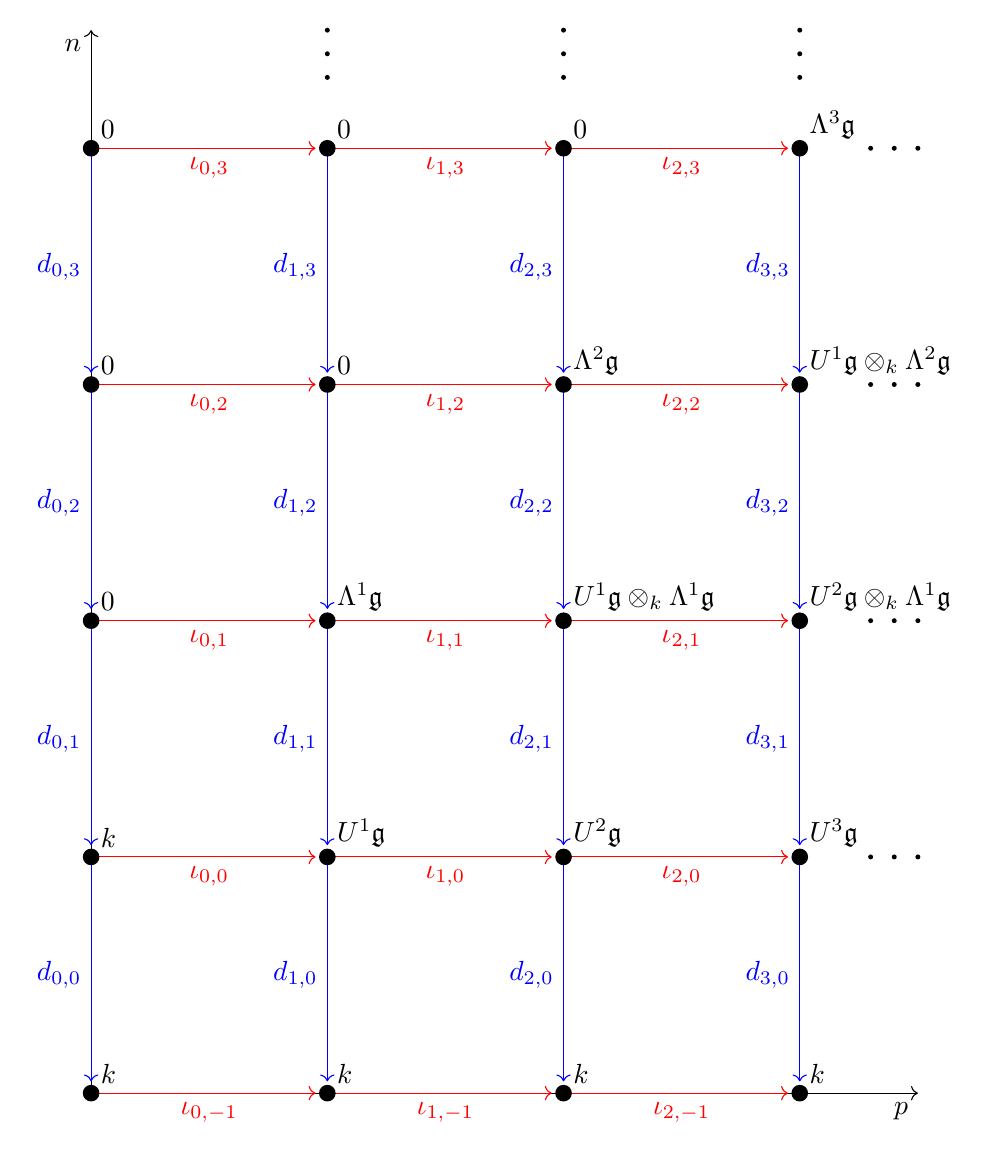
\begin{tikzpicture}[scale=3]  % Increased scale for better visibility
        % Grid dimensions
        \def\maxn{3} % Adjust as needed
        \def\minn{-1} % New minimum n value
        \def\maxp{3} % Adjust as needed

        % Drawing the axes
        \draw[->] (0,-1) -- (\maxp+0.5,-1) node[anchor=north east] {$p$};
        \draw[->] (0,-1) -- (0,\maxn+0.5) node[anchor=north east] {$n$};

        % Drawing the lattice points, labels, and differential maps
        \foreach \n in {\minn,...,\maxn} {
          \foreach \p in {0,...,\maxp} {
            % Calculate p - n
            \pgfmathtruncatemacro{\diff}{\p - \n}

            % Conditional structure for labeling
            \ifnum\n=-1
              \node[anchor=south west, black] at (\p,\n) {$k$}; % Special row for n = -1
            \else
              \ifnum\n>\p
                \node[anchor=south west, black] at (\p,\n) {0}; % Label as zero if n > p
              \else
                \ifnum\n=\p
                  \ifnum\n=0 % Special case for M_{0,0} = k
                    \node[anchor=south west, black] at (\p,\n) {$k$};
                  \else % Special case for diagonal (Lambda^n g)
                    \node[anchor=south west, black] at (\p,\n) {$\Lambda^\n \mathfrak{g}$};
                  \fi
                \else
                  \ifnum\n=0 % Special case for p-axis (p > 0, n = 0)
                    \node[anchor=south west, black] at (\p,\n) {$U^{\p}\mathfrak{g}$};
                  \else % General case
                    \node[anchor=south west, black] at (\p,\n) {$U^{\diff}\mathfrak{g} \otimes_k \Lambda^\n \mathfrak{g}$};
                  \fi
                \fi
              \fi
            \fi

            % Draw differential maps (vertical arrows)
            \ifnum\n>-1
              \draw[->, blue] (\p,\n) -- (\p,\n-0.95); % Vertical differential
              \node[anchor=east, blue] at (\p,\n-0.5) {$d_{\p,\n}$};
            \fi
            \ifnum\p<\maxp
              \draw[->, red] (\p,\n) -- (\p+0.95,\n); % Horizontal inclusion
              \node[anchor=north, red] at (\p+0.5,\n) {$\iota_{\p,\n}$};
            \fi


            % Draw lattice points
            \fill (\p,\n) circle (1pt);

          }
        }

        % Adding dots to indicate continuation
        \foreach \n in {0,...,\maxn} {
          \fill (\maxp+0.3,\n) circle (0.3pt);  % Dots on the right side
          \fill (\maxp+0.4,\n) circle (0.3pt);
          \fill (\maxp+0.5,\n) circle (0.3pt);
        }
        \foreach \p in {1,...,\maxp} {
          \fill (\p,\maxn+0.3) circle (0.3pt);  % Dots on the top side
          \fill (\p,\maxn+0.4) circle (0.3pt);
          \fill (\p,\maxn+0.5) circle (0.3pt);
        }
      \end{tikzpicture}
    \end{center}
    \caption{A small portion of $ F_{p, n} $ for $ -1 \leq n \leq 3 $ and $ 0 \leq p \leq 3 $ where the blue arrows are the induced differential maps on $ F_p $ and the red arrows are the inclusion maps. Notice that $ F_p $ is the sum of the $ F_{p,n} $'s along the vertical.}\label{fig:filtrationf}
  \end{figure}
  The filtration can be visualized on a 2d lattices as shown in Figure~\ref{fig:filtrationf}. Note that we define the maps $ d_{p, 0}:F_{p, 0} \to F_{p, -1} $ to be the restriction of the augmentation map, i.e., $ d_{p, 0} = \epsilon|_{U^{p}\mathfrak{g}} $. Moreover, for $ n>0 $ we let $ d_{p, n}: F_{p, n} \to F_{p, n-1} $ be the restriction of $ d_n $ to $ F_{p,n} $ and as $ d_n(F_{p, n}) \subset F_{p, n-1} $ we have a well defined boundary map which squares to zero and hence makes $ F_p $ into a chain complex.

  For $ n\geq 0 $ the inclusion $\iota'_{k-1}: U^{k-1}\mathfrak{g} \to U^{k}\mathfrak{g} $ extends to an inclusion $ \iota_{p, n}: F_{p, n} \to F_{p+1, n} $ which is natural with respect to the boundary map $ d_{p, n} $ (we set $ \iota_{-1, p} $ to be the identity on $ k $). We thus have an induced map of chain complexes $ \iota_p: F_p \to F_{p + 1} $. This gives rice to a sequence of inclusions $ F_0 \subset F_1 \subset \cdots \subset F_p \subset \cdots $ with direct limit equal to $ \bigcup_{p = 0}^{\infty} F_p = V_{*}(\mathfrak{g}) \xrightarrow{\epsilon} k $. As homology preserves direct limits we then have that
  \begin{align*}
    H_*\left( V_{*}(\mathfrak{g}) \xrightarrow{\epsilon} k\right) &= H_* \left( \bigcup_{p = 0}^{\infty} F_p \right) \\
                                                                  &= H_* \left( \varinjlim{F_p} \right) \\
                                                                  &= \varinjlim{H_*(F_p)}
  \end{align*}
  and so if we can show that $ H_*(F_p) = 0 $ then we are done.

  To this end, for $ p \geq 1 $ we define a new chain complex $ W_p = \text{coker}(\iota_{p - 1}) $ which more explicitly is given by
  \begin{equation}
    W_{p, n} = \begin{cases}
      F_{p, n}/F_{p-1, n}, &\text{ if } n \geq 0,\\
      0, &\text{ else}.
    \end{cases}
  \end{equation}

  This gives us a short exact sequence of chain complexes:
  \begin{equation}
    \label{eq:ses}
    0 \to F_{p - 1} \xrightarrow{\iota} F_p \xrightarrow{\pi} W_p \to 0.
  \end{equation}
  Note that, since $ \Lambda^{n}\mathfrak{g} $ is a free $ k $-module, tensoring with $ \Lambda^{n}\mathfrak{g} $ preserves exactness and so for $ 0\leq n \leq p $ we have
  \begin{equation}
    W_{p, n} = (U^{p - n}\mathfrak{g}\otimes_k \Lambda^{n}\mathfrak{g}) /(U^{p - n - 1}\mathfrak{g}\otimes_k \Lambda^{n}\mathfrak{g}) \cong (U^{p - n}\mathfrak{g} /U^{p - n - 1}\mathfrak{g})\otimes_k \Lambda^{n}\mathfrak{g}.
  \end{equation}

  We can visualize the modules $ W_{p, n} $ on a 2d lattice as done in Figure~\ref{fig:filtration} where we see that $ W_{p, n} $ is zero above the diagonal. Note especially that along the diagonal ($ p = n $) we have $ W_{p, n} = \Lambda^{n}\mathfrak{g} $ and on the $ p $-axis $ \Lambda^{0}\mathfrak{g} = k $ so that we end up with just $ U^{p}\mathfrak{g}/U^{p-1}\mathfrak{g} $.

  Now, if $ \{e_{\alpha}\} $ is a basis for $ \mathfrak{g} $ and $ I = (\alpha_1, \ldots, \alpha_{p - n}) $ is an increasing sequence then $ U^{p - n}\mathfrak{g}/U^{p - n -1}\mathfrak{g} $ is the free $ k $-module generated by the image of basis elements $ e_{I} $, denoted as $ \overline{e}_{I} $. Therefore, if $ J = (\beta_1, \ldots, \beta_n) $ is a strictly increasing sequence, then the differential $ d_{p, n}: W_{p, n} \to W_{p, n- 1} $ is given on basis elements $ \overline{e}_{I} \otimes e^{J} $ as follows.
  \begin{align*}
    d_n(\overline{e}_{I} \otimes e^{J}) &= \sum_{i = 1}^{n} (-1)^{i + 1} \overline{e}_{(I, \beta_i)} \otimes \wedge(e_{\beta_1}, \widehat{e}_{\beta_i}, e_{\beta_n}) \\
                                        &\quad+ \sum_{i < j} (-1)^{i + j} \overline{e}_{I} \otimes [e_{\beta_i}, e_{\beta_j}] \wedge(e_{\beta_1}, e_{\beta_i}, e_{\beta_j}, e_{\beta_n}) \\
                                        &= \sum_{i = 1}^{n} (-1)^{i + 1} \overline{e}_{(I, \beta_i)} \otimes \wedge(e_{\beta_1}, \widehat{e}_{\beta_i}, e_{\beta_n})
  \end{align*}
  as $ \overline{e}_{I} = 0 $ in $ U^{p - n + 1}\mathfrak{g}/U^{p - n}\mathfrak{g} $. Another important fact is that if $ I = (\alpha_1', \alpha_2') $ with $ \alpha_2' < \alpha_1' $, then
  \begin{equation}
    e_{(\alpha_1', \alpha_2')} = e_{(\alpha_2', \alpha_1')} - [e_{\alpha_1'}, e_{\alpha_2'}]
  \end{equation}
  so that in $ U^2\mathfrak{g}/U^{1}{\mathfrak{g}} $ we have
  \begin{equation}
    \overline{e}_{(\alpha_1', \alpha_2')} = \overline{e}_{(\alpha_1, \alpha_2)}
  \end{equation}
  where $ (\alpha_1, \alpha_2) = (\alpha_2', \alpha_1') $. More generally we therefore have that if $ I' = (\alpha_1', \ldots, \alpha_k') $ is any sequence, not necessarily increasing, and $ I = (\alpha_1, \ldots, \alpha_k) $ is an increasing version of $ I' $, then
  \begin{equation}
    \overline{e}_{I'} = \overline{e}_{I}
  \end{equation}
  in $ U^{k}\mathfrak{g}/U^{k - 1}\mathfrak{g} $.

  \begin{figure}[t]
    \begin{center}
      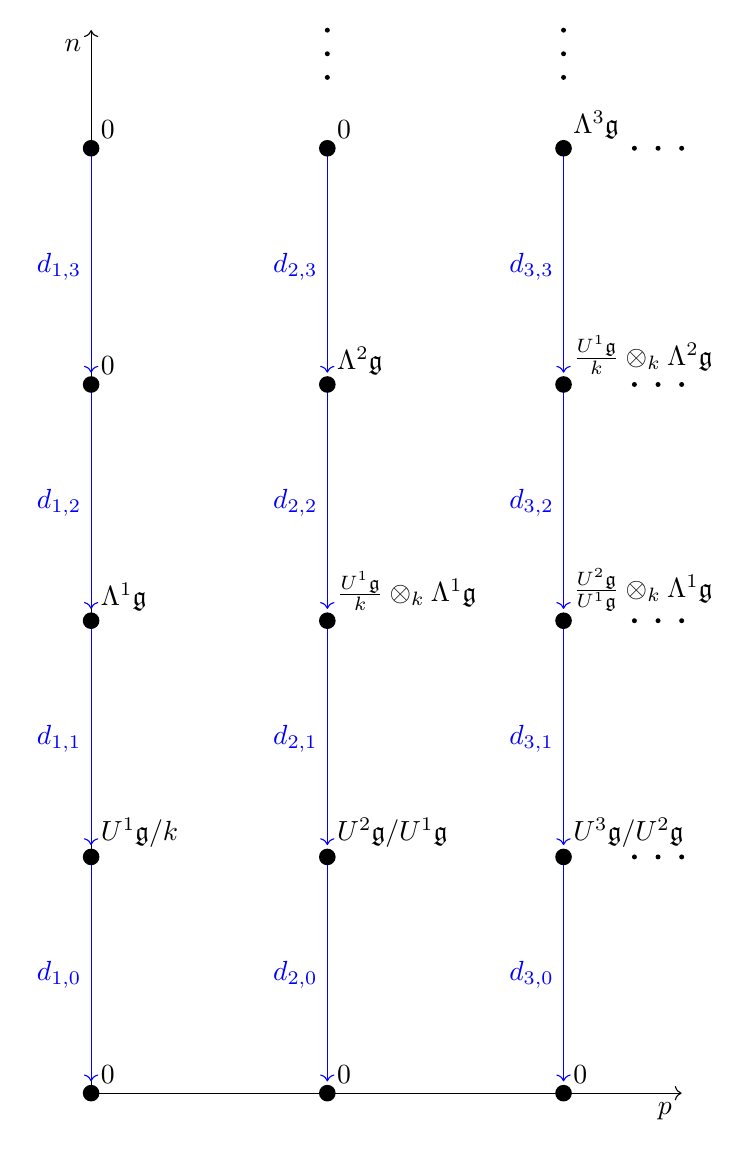
\begin{tikzpicture}[scale=3]  % Increased scale for better visibility
        % Grid dimensions
        \def\maxn{3} % Adjust as needed
        \def\minn{-1} % New minimum n value
        \def\maxp{3} % Adjust as needed
        \def\minp{1}  % Define minimum p value

        % Drawing the axes
        \draw[->] (\minp,-1) -- (\maxp+0.5,-1) node[anchor=north east] {$p$};
        \draw[->] (\minp,-1) -- (\minp,\maxn+0.5) node[anchor=north east] {$n$};

        % Drawing the lattice points, labels, and differential maps
        \foreach \n in {\minn,...,\maxn} {
          \foreach \p in {\minp,...,\maxp} {
            % Calculate p - 1 - n
            \pgfmathtruncatemacro{\diff}{\p - 1 - \n}
            \pgfmathtruncatemacro{\difff}{\p - \n}

            % Conditional structure for labeling
            \ifnum\n=-1
              \node[anchor=south west, black] at (\p,\n) {0}; % Special row for n = -1
            \else
              \ifnum\n>\p
                \node[anchor=south west, black] at (\p,\n) {0}; % Label as zero if n > p
              \else
                \ifnum\n=\p
                  \ifnum\n=0 % Special case for M_{0,0} = k
                    \node[anchor=south west, black] at (\p,\n) {$k$};
                  \else % Special case for diagonal (Lambda^n g)
                    \node[anchor=south west, black] at (\p,\n) {$\Lambda^\n \mathfrak{g}$};
                  \fi
                \else
                  \ifnum\n=0 % Special case for p-axis (p > 0, n = 0)
                    \ifnum\p=1
                      \node[anchor=south west, black] at (\p,\n) {$U^{\p}\mathfrak{g}/k$};
                    \else
                      \node[anchor=south west, black] at (\p,\n) {$U^{\p}\mathfrak{g}/U^{\diff}\mathfrak{g} $};
                    \fi
                  \else % General case
                    \ifnum\diff=0
                      \node[anchor=south west, black] at (\p,\n) {$\frac{U^{\difff}\mathfrak{g}}{k} \otimes_k \Lambda^\n \mathfrak{g}$};
                    \else
                      \node[anchor=south west, black] at (\p,\n) {$\frac{U^{\difff}\mathfrak{g}}{U^{\diff}\mathfrak{g}} \otimes_k \Lambda^\n \mathfrak{g}$};
                    \fi
                  \fi
                \fi
              \fi
            \fi

            % Draw differential maps (vertical arrows)
            \ifnum\n>-1
              \draw[->, blue] (\p,\n) -- (\p,\n-0.95); % Vertical differential
              \node[anchor=east, blue] at (\p,\n-0.5) {$d_{\p,\n}$};
            \fi

            % Draw lattice points
            \fill (\p,\n) circle (1pt);
          }
        }

        % Adding dots to indicate continuation
        \foreach \n in {0,...,\maxn} {
          \fill (\maxp+0.3,\n) circle (0.3pt);  % Dots on the right side
          \fill (\maxp+0.4,\n) circle (0.3pt);
          \fill (\maxp+0.5,\n) circle (0.3pt);
        }
        \foreach \p in {2,...,\maxp} {
          \fill (\p,\maxn+0.3) circle (0.3pt);  % Dots on the top side
          \fill (\p,\maxn+0.4) circle (0.3pt);
          \fill (\p,\maxn+0.5) circle (0.3pt);
        }
      \end{tikzpicture}
    \end{center}
    \caption{A small portion of $ W_{p, n} $ for $ 1 \leq p \leq 3 $ and $ -1 \leq n \leq 3 $ where the blue arrows are the induced differential maps on $ W_p $ which you get from the maps $ d_{p, n}:F_{p, n} \to F_{p, n-1} $. The chain complexes $ W_p $ are the direct sum of the components along the vertical direction.}\label{fig:filtration}
  \end{figure}


  Now, if we can show that $ W_p $ has trivial homology, then the long exact sequence induced from the short exact sequence in \ref{eq:ses} gives us that $ H_*(F_{p}) \cong H_{*}(F_{p-1}) $ for all $ p $. Since $ F_0 $ is just the trivial complex $ 0 \to k \to k \to 0 $ we have that $ H_*(F_0) = 0 $ and hence this would imply that $ H_*(F_p) = 0 $ for all $ p $ leading us to conclude that
  \begin{equation}
    H_*\left( V_*(\mathfrak{g})\xrightarrow{\epsilon} k \right) = \varinjlim{H_*(F_p)} = 0.
  \end{equation}

  What remains to show then is that $ H_*(W_p) = 0 $ for all $ p \geq 1 $. We do this explicitly by creating a chain homotopy $ s_{p, *}: W_{p, *} \to W_{p, *+1} $ between the identity and the zero map. Therefore, let $ I=(\alpha_1, \ldots, \alpha_{p - n} ) $ be an increasing sequence and $ J = (\beta_1, \ldots, \beta_n) $ a strictly increasing sequence. We then define $ s_{p, n} $ on basis elements $ \overline{e}_{I} \otimes e^{J} $ as follows:
  \begin{equation}
    s_{p, n}(\overline{e}_I \otimes e^{J}) = \begin{cases}
      (-1)^{n}\overline{e}_{(\alpha_1, \ldots, \alpha_{p - n - 1})}\otimes e^{(J, \alpha_{p - n})}, &\text{ if } \alpha_{p - n} > \beta_n\\
      0, &\text{ else.}
    \end{cases}
  \end{equation}
  Our goal is to show that
  \begin{equation}
    s_{p, n-1}d_{p, n} + d_{p, n+1}s_{p, n} = 1_{W_{p,n}}.
  \end{equation}
  Hence, let $ I = (\alpha_1, \ldots, \alpha_{p -n}) $ be an increasing sequence and $ J = (\beta_1, \ldots, \beta_n) $ a strictly increasing sequence. There are then two cases two consider, either $ \alpha_{p - n} > \beta_n $ or $ \alpha_{p - n} \leq \beta_n $. Assume first that $ \alpha_{p -n} > \beta_n $. We then have that
  \begin{align*}
    (s_{p, n-1}d_{p, n} + d_{p, n+1}s_{p, n})(\overline{e}_{I} \otimes e^{J}) &= s_{p, n-1}\left( \sum_{i = 1}^{n} (-1)^{i + 1}\overline{e}_{(I, \beta_i)} \otimes \wedge\left(e_{\beta_1}, \widehat{e}_{\beta_i}, e_{\beta_n}\right) \right) \\
                                                                            &\quad + d_{p, n-1}\left( (-1)^{n}\overline{e}_{(\alpha_1, \ldots, \alpha_{p-n-1})} \otimes e^{(J, \alpha_{p -n})} \right) \\
                                                                            &= \sum_{i = 1}^{n} (-1)^{i + n} \overline{e}_{(\alpha_1, \ldots, \alpha_{p - n - 1}, \beta_i)} \otimes \wedge\left(e_{\beta_1}, \widehat{e}_{\beta_i}, e_{\beta_n}, e_{\alpha_{p-n}} \right) \\
                                                                            &\quad + \sum_{i = 1}^{n} (-1)^{i + n + 1}\overline{e}_{(\alpha_1, \ldots, \alpha_{p-n-1}, \beta_i)} \otimes \wedge \left( e_{\beta_1}, \widehat{e}_{\beta_i}, e_{\beta_n}, e_{\alpha_{p - n}} \right) \\
                                                                            &\quad + \overline{e}_{I} \otimes e^{J} \\
                                                                            &= \overline{e}_{I} \otimes e^{J},
  \end{align*}
  where we use the fact that $ \alpha_{p - n} > \beta_i $ and so $ \overline{e}_{\alpha_1, \ldots, \alpha_{p - n}, \beta_i} = \overline{e}_{\alpha_1, \ldots, \beta_i, \alpha_{p - n}} $ in accordance with an earlier remark. The only important thing in the definition of $ s_{p, n} $ on basis elements is that the rightmost element in $ I $ is the largest one which is why we can apply $ s_{p, n-1} $ to $ \overline{e}_{(\alpha_1, \ldots, \alpha_{p -n - 1}, \beta_i, \alpha_{p -n})} \otimes \wedge \left( e_{\beta_1}, \widehat{e}_{\beta_i}, e_{\beta_n} \right) $ without much problem.

  On the other hand, assume that $ \alpha_{p - n} \leq \beta_n $. We then have that
  \begin{equation}
    s_{p, n}\left( e_{I} \otimes e^{J} \right) = 0
  \end{equation}
  and
  \begin{equation}
    s_{p, n -1} \left( \overline{e}_{(I, \beta_i)} \otimes \wedge \left( e_{\beta_1}, \widehat{e}_{\beta_i}, e_{\beta_n} \right) \right) = 0
  \end{equation}
  except for $ i = n $ where we have
  \begin{equation}
    s_{p, n -1}\left( e_{(I, \beta_n)} \otimes e^{(\beta_1, \ldots, \beta_{n - 1})} \right) = (-1)^{n - 1} \overline{e}_{I} \otimes e^{J}.
  \end{equation}
  From this it follows that
  \begin{align*}
    (s_{p, n-1}d_{p, n} + d_{p, n+1}s_{p, n})(\overline{e}_{I} \otimes e^{J}) &=  s_{p, n-1}\left( \sum_{i = 1}^{n} (-1)^{i + 1}\overline{e}_{(I, \beta_i)} \otimes \wedge\left(e_{\beta_1}, \widehat{e}_{\beta_i}, e_{\beta_n}\right) \right) + d_{p, n-1}(0) \\
                                                                              &= \sum_{i = 1}^{n} (-1)^{i + 1}s_{p, n-1}\left(\overline{e}_{(I, \beta_i)} \otimes \wedge\left(e_{\beta_1}, \widehat{e}_{\beta_i}, e_{\beta_n}\right)\right) \\
                                                                              &= (-1)^{n + 1 + n -1} \overline{e}_{I} \otimes e^{J} \\
                                                                              &= \overline{e}_{I} \otimes e^{J}
  \end{align*}
  as desired. We therefore see that $ s_{p, *}: W_{p, *} \to W_{p, *+1} $ is a chain homotopy between the identity and zero map on $ W_p $ which means that $ H_*(W_p) = 0 $. By earlier remarks this then implies that
  \begin{equation}
    H_*\left( V_*(\mathfrak{g})\xrightarrow{\epsilon} k \right) = 0
  \end{equation}
  showing that $ V_*(\mathfrak{g})\xrightarrow{\epsilon} k $ indeed is a projective resolution of $ k $ considered as a trivial $ \mathfrak{g} $-module (equivalently trivial $ U\mathfrak{g} $-module).
\end{proof}

\begin{corollary}[\cite{weibel1994homological}]
  \label{cor:cohom}
  If $ M $ is a right $ \mathfrak{g} $-module, then the homology modules $ H_*(\mathfrak{g}, M) $ are the homology of the chain complex
  \begin{equation}
    M \otimes_{U\mathfrak{g}} V_{*}(\mathfrak{g}) = M \otimes_{U\mathfrak{g}} U\mathfrak{g} \otimes_k \Lambda^{*}\mathfrak{g} = M \otimes_k \Lambda^{*}\mathfrak{g}.
  \end{equation}
  Similarly, if $ M $ is a left $ \mathfrak{g} $-module, then the cohomology modules $ H^{*}(\mathfrak{g}, M) $ are the cohomology of the cochain complex
  \begin{equation}
    \text{Hom}_{\mathfrak{g}\text{-}\mathbf{Mod}}(V_*(\mathfrak{g}), M) = \text{Hom}_{\mathfrak{g}\text{-}\mathbf{Mod}}(U\mathfrak{g} \otimes_k \Lambda^{*}\mathfrak{g}, M) \cong \text{Hom}_{k\text{-}\mathbf{Mod}}(\Lambda^{*}\mathfrak{g}, M).
  \end{equation}
  In this complex, an $ n $-cochain $ f: \Lambda^{n}\mathfrak{g} \to M $ is just an alternating $ k $-multilinear of $ n $ variables in $ \mathfrak{g} $, taking values in $ M $. The coboundary $ \delta f $ of such an $ n $-cochain is the $ (n +1) $-cochain given by
  \begin{align*}
    \delta f(e_{\alpha_1}, \ldots, e_{\alpha_n}, e_{\alpha_{n + 1}}) = &\sum_{i = 1}^{n} (-1)^{i + 1} e_{\alpha_i}f(e_{\alpha_1}, \ldots, \widehat{e}_{\alpha_i}, \ldots, e_{\alpha_n}, e_{\alpha_{n + 1}}) \\
                                                                       &+ \sum_{i < j} (-1)^{i + j} f \left( [e_{\alpha_i}, e_{\alpha_{j}}], e_{\alpha_1}, \ldots, \widehat{e}_{\alpha_i}, \ldots, \widehat{e}_{\alpha_j}, \ldots, e_{\alpha_n}, e_{\alpha_{n + 1}} \right).
  \end{align*}
\end{corollary}
% subsection The Chevalley-Eilenberg Complex (end)

\subsection{$ H^2 $ and extensions} % (fold)
\label{sub:H^2 and extensions}
Corollary~\ref{cor:cohom} gives us a concrete and practical way of calculating the Lie algebra (co)homology for a wide array of Lie algebras $ \mathfrak{g} $ and $ \mathfrak{g} $-modules $ M $. However, in the special case of wanting to compute $ H^2(\mathfrak{g}, M) $ we can classify the cohomology in another way, namely as equivalence classes of Lie algebra extensions of $ \mathfrak{g} $ by $ M $. For this to make sense we need to understand what we mean by such an extension.
\begin{definition}[Extension of a Lie algebra]
  Let $ \mathfrak{g} $ and $ \mathfrak{h} $ be two Lie algebras. An \textbf{extension} of $ \mathfrak{g} $ by $ \mathfrak{h} $ is a short exact sequence of Lie algebras:
  \begin{equation}
    \label{eq:lieextension}
    0 \to \mathfrak{h} \xrightarrow{i} \mathfrak{e} \xrightarrow{p} \mathfrak{g} \to 0.
  \end{equation}
  Two such extensions of $ \mathfrak{g} $ by $ \mathfrak{h} $ are said to be equivalent if there exist a Lie algebra homomorphism $ \varphi: \mathfrak{e} \to \mathfrak{e}' $ which makes the following diagram commute:
  \[\begin{tikzcd}
	  0 & {\mathfrak{h}} & {\mathfrak{e}} & {\mathfrak{g}} & 0 \\
	  0 & {\mathfrak{h}} & {\mathfrak{e}'} & {\mathfrak{g}} & 0.
	  \arrow[Rightarrow, no head, from=1-4, to=2-4]
	  \arrow["\varphi", from=1-3, to=2-3]
	  \arrow[from=1-1, to=1-2]
	  \arrow["i", from=1-2, to=1-3]
	  \arrow["p", from=1-3, to=1-4]
	  \arrow[from=1-4, to=1-5]
	  \arrow["{i'}"', from=2-2, to=2-3]
	  \arrow["{p'}"', from=2-3, to=2-4]
	  \arrow[from=2-1, to=2-2]
	  \arrow[from=2-4, to=2-5]
	  \arrow[Rightarrow, no head, from=1-2, to=2-2]
  \end{tikzcd}\]
  The five-lemma implies that $ \varphi $ must necessarily be an isomorphism.
\end{definition}

\begin{definition}[Split extension]
  An extension of the form in \ref{eq:lieextension} is called \textbf{split} if there exists a Lie algebra homomorphism $ \tau: \mathfrak{g} \to \mathfrak{e} $ such that $ p \circ \tau = 1_\mathfrak{g} $.
\end{definition}

Before we properly define what we mean by an extension of $ \mathfrak{g} $ by a $ \mathfrak{g} $-module $ M $ we need to talk about semidirect products.
\begin{definition}[Semidirect product]
  Let $ \mathfrak{g} $ be a Lie algebra and $ M $ a $ \mathfrak{g} $-module. The semidirect product of $ M $ and $ \mathfrak{g} $, denoted $ M \rtimes \mathfrak{g} $, is the Lie algebra with underlying $ k $-module structure $ M \oplus \mathfrak{g} $ and Lie bracket given by
  \begin{equation}
    [(m, x), (n, y)] = \left(xn - ym, [x, y]\right).
  \end{equation}
\end{definition}
Now, let $ M $ be an abelian Lie algebra and $ \mathfrak{e} $ and extension of $ \mathfrak{g} $ by $ M $. This means we have a short exact sequence of the form
\begin{equation}
  0 \to M \xrightarrow{i} \mathfrak{e} \xrightarrow{p} \mathfrak{g} \to 0.
\end{equation}
We can then give $ M $ a $ \mathfrak{g} $-module structure as follows. For $ x \in \mathfrak{g} $ and $ m \in M $ let
\begin{equation}
  xm = i^{-1}\left( [\pi^{-1}(x), i(m)] \right).
\end{equation}
To see why this is well defined, suppose $ \pi(e) = x = \pi(e') $. Then $ \pi(e - e') = 0 $ and by exactness there then exists an $ m' \in M $ such that $ i(m')=e - e' $. However, this implies that
\begin{align*}
  i^{-1}\left( [e, i(m)] \right) - i^{-1}(\left( [e', i(m)] \right)) &= i^{-1}\left( [e - e', i(m)] \right) \\
                                                                     &= i^{-1}(i([m', m])) \\
                                                                     &= i^{-1}(i(0)) \\
                                                                     &= 0
\end{align*}
showing that $ xm $ is well defined. The interesting case is when $ M $ already has a $ \mathfrak{g} $-module. In this case we can form the extension of $ \mathfrak{g} $ by $ M $ by taking the semidirect product of $ M $ and $ \mathfrak{g} $ and give $ M $ a new $ \mathfrak{g} $-module structure from $ M \rtimes \mathfrak{g} $.
\begin{lemma}
  Let $ M $ be a $ \mathfrak{g} $-module. Then the induced $ \mathfrak{g} $-module structure on $ M $ which we get from the short exact sequence
  \begin{equation}
    0 \to M \xrightarrow{\iota} M \rtimes \mathfrak{g} \xrightarrow{\pi} \mathfrak{g} \to 0
  \end{equation}
  coincides with the original $ \mathfrak{g} $-module structure.
\end{lemma}
\begin{proof}
  We choose $ (0, x) $ as the representative for $ \pi^{-1}(x) $. We then have that
  \begin{align*}
    \iota^{-1}\left( [\pi^{-1}(x), i(m)] \right) &= \iota^{-1}\left( [(0,x), (m, 0)] \right) \\
                                             &= \iota^{-1}\left(xm - 0\cdot0, [0,0]\right) \\
                                             &= \iota^{-1}((xm, 0)) \\
                                             &= xm
  \end{align*}
  showing that they coincide.
\end{proof}
We can now state the theorem we want to show.

\begin{theorem}
  \label{thm:equivalence}
  Let $ \mathfrak{g} $ be a Lie algebra over $ k $ and $ M $ a $ \mathfrak{g} $-module. Then the elements of $ H^2(\mathfrak{g}, M) $ are in a natural one-to-one correspondence with the set of equivalence classes of Lie algebra extensions of $ \mathfrak{g} $ by $ M $ that induce the same fixed $ \mathfrak{g} $-module structure.
\end{theorem}
We delay the proof of this theorem to follow the path suggested in \cite[Exercise 7.7.5]{weibel1994homological} and prove some lemmas first.

\begin{lemma}
  Let $ M $ be a $ \mathfrak{g} $-module. If $ 0 \to M \xrightarrow{i} \mathfrak{e} \xrightarrow{p} \mathfrak{g} \to 0 $ is an extension of Lie algebras that induce the same $ \mathfrak{g} $-module structure on $ M $, and $ \sigma: \mathfrak{g} \to \mathfrak{e} $ is a $ k $-module splitting of $ p $ (such a splitting exists as $ \mathfrak{g} $ is free) then the Lie algebra structure on $ \mathfrak{e} \cong M \oplus \mathfrak{g} $ may be described by an alternating $ k $-bilinear function $ \omega: \mathfrak{g} \times \mathfrak{g} \to M $ defined by
  \begin{equation}
    \omega(x,y) = i^{-1}\left([\sigma(x), \sigma(y)] - \sigma \left( [x, y] \right)\right), \quad\quad \forall x,y \in \mathfrak{g}.
  \end{equation}
  Moreover, $ \omega $ is a cochain, meaning that $ \delta \omega = 0 $.
\end{lemma}
\begin{proof}
  First of all, notice that the definition of $ \omega $ makes sense as applying $ p $ to the inner argument of $ i^{-1} $ gives $ 0 $ and hence there must exist an element $ m \in M $ such that $ i(m)=i(\omega(x,y)) $.

  Next, some conventions: let $ xm $ denote the original $ \mathfrak{g} $-module action of $ \mathfrak{g} $ on $ M $ and let $ x_{\mathfrak{e}} m $ denote the $ \mathfrak{g} $-module action of $ \mathfrak{g} $ on $ M $ induced by the Lie algebra extension. By assumption we then have $ x_{\mathfrak{e}}m = xm $ for all $ x \in \mathfrak{g} $ and $ m \in M $. Next, let
  \begin{equation}
    0 \to M \xrightarrow{\iota} M \rtimes \mathfrak{g} \xrightarrow{\pi} \mathfrak{g} \to 0
  \end{equation}
  be the short exact sequence of Lie algebras you get from taking the semidirect product of $ M $ and $ \mathfrak{g} $.

  The $ k $-module isomorphism $ \psi: M \oplus \mathfrak{g} \to \mathfrak{g} $ is then given on elements by
  \begin{equation}
    \psi(m , x) = i(m) + \sigma(x),\quad \forall (m,x) \in M \oplus \mathfrak{g}
  \end{equation}
  and
  \begin{equation}
    \psi^{-1}(d) = (i^{-1}(d - \sigma(p(d))), p(d)), \quad \forall d \in \mathfrak{e}.
  \end{equation}
  This implies that the Lie algebra structure on $ M \oplus \mathfrak{g} $ is given by
  \begin{equation}
    [(m, x), (n, y)] = \psi^{-1}\left( [\psi(m, x), \psi(n, y)] \right),
    \quad \forall (m,x),(n,y) \in M \oplus \mathfrak{g}
  .\end{equation}
  Expanding this out we have
  \begin{align*}
    [(m, x), (n, y)] &= \psi^{-1}\left( [i(m) + \sigma(x),  i(n) + \sigma(y)] \right) \\
                     &= \psi^{-1}\left( i([m, n]) + [\sigma(x), i(n)] - [\sigma(y), i(m)] + [\sigma(x), \sigma(y)] \right) \\
                     &=\psi^{-1}\left( i(x_{\mathfrak{e}} n - y_{\mathfrak{e}} m ) + [\sigma(x), \sigma(y)] \right) \\
                     &= (x_{\mathfrak{e}}n - y_{\mathfrak{e}}m + i^{-1}(\left( [\sigma(x), \sigma(y)] \right) - \sigma([x, y])), [x, y])\\
                     &= (x_{\mathfrak{e}}n - y_{\mathfrak{e}}m +\omega(x,y), [x, y])
  \end{align*}
  showing that the Lie algebra structure on $ M \oplus \mathfrak{g} \cong \mathfrak{e} $ indeed is given by the $ k $-bilinear alternating function
  \begin{equation}
    \omega(x,y) = i^{-1}([\sigma(x), \sigma(y)] - \sigma([x,y])).
  \end{equation}

  Next to see that $ \delta \omega = 0 $, let $ x,y,z \in \mathfrak{g} $. In the following we shall use $ \sigma(x), \sigma(y), \sigma(z) $ as canditates for $ p^{-1}(x)$, $p ^{-1}(y), $ and $ p ^{-1}(z) $ respectively. Corollary~\ref{cor:cohom} now implies that
  \begin{align*}
    \delta \omega (x,y,z) &= x\omega(y, z) - y\omega(x, z) + z\omega(x,y) \\
                          &\quad -\omega([x,y], z) + \omega([x,z], y) - \omega([y,z], x) \\ \\
                          &= x i^{-1}([\sigma(y), \sigma(z)] - \sigma([y,z])) \\
                          &\quad -yi^{-1}([\sigma(x), \sigma(z)] - \sigma([x,z])) \\
                          &\quad +zi^{-1}([\sigma(x), \sigma(y)]- \sigma([x,y])) \\
                          &\quad - i^{-1}([\sigma([x, y]), \sigma(z)]-\sigma([[x,y], z])) \\
                          &\quad + i^{-1}([\sigma([x, z]), \sigma(y)] -\sigma([[x,z], y])) \\
                          &\quad - i^{-1}([\sigma([y, z]), \sigma(x)] -\sigma([[y,z], x])) \\ \\
                          &= x_{\mathfrak{e}}i^{-1}([\sigma(y), \sigma(z)] - \sigma([y,z])) \\
                          &\quad -y_{\mathfrak{e}}i^{-1}([\sigma(x), \sigma(z)] - \sigma([x,z])) \\
                          &\quad +z_{\mathfrak{e}}i^{-1}([\sigma(x), \sigma(y)]- \sigma([x,y])) \\
                          &\quad - i^{-1}([\sigma([x, y]), \sigma(z)]-\sigma([[x,y], z])) \\
                          &\quad + i^{-1}([\sigma([x, z]), \sigma(y)] -\sigma([[x,z], y])) \\
                          &\quad - i^{-1}([\sigma([y, z]), \sigma(x)] -\sigma([[y,z], x])) \\ \\
                          &= i^{-1}([\sigma(x), [\sigma(y), \sigma(z)]] - [\sigma(x), \sigma([y, z])]) \\
                          &\quad - i^{-1}([\sigma(y), [\sigma(x), \sigma(z)]] - [\sigma(y), \sigma([x, z])]) \\
                          &\quad + i^{-1}([\sigma(z), [\sigma(x), \sigma(y)]] - [\sigma(z), \sigma([x, y])]) \\
                          &\quad - i^{-1}([\sigma([x, y]), \sigma(z)]-\sigma([[x,y], z]) \\
                          &\quad + i^{-1}([\sigma([x, z]), \sigma(y)] -\sigma([[x,z], y])) \\
                          &\quad - i^{-1}([\sigma([y, z]), \sigma(x)] -\sigma([[y,z], x])) \\ \\
                          &= i^{-1}([\sigma(x), [\sigma(y), \sigma(z)]] - [\sigma(x), \sigma([y, z])] \\
                          &\quad\quad\quad - [\sigma(y), [\sigma(x), \sigma(z)]] + [\sigma(y), \sigma([x, z])] \\
                          &\quad\quad\quad + [\sigma(z), [\sigma(x), \sigma(y)]] - [\sigma(z), \sigma([x, y])] \\
                          &\quad\quad\quad - [\sigma([x, y]), \sigma(z)]+\sigma([[x,y], z]) \\
                          &\quad\quad\quad + [\sigma([x, z]), \sigma(y)] -\sigma([[x,z], y]) \\
                          &\quad\quad\quad - [\sigma([y, z]), \sigma(x)] +\sigma([[y,z], x]))
  \end{align*}
  The Jacobi identity implies that both
  \begin{align*}
    \sigma([[x,y], z]) - \sigma([[x, z], y]) + \sigma([[y,z], x]) &= \sigma([[x,y], z]) + \sigma([[z, x], y]) + \sigma([[y,z], x]) \\&= 0
  \end{align*}
  and
  \begin{align*}
    &[\sigma(x), [\sigma(y), \sigma(z)]] -
    [\sigma(y), [\sigma(x), \sigma(z)]] +
    [\sigma(z), [\sigma(x), \sigma(y)]]\\ &=
    [\sigma(x), [\sigma(y), \sigma(z)]] +
    [\sigma(y), [\sigma(z), \sigma(x)]] +
    [\sigma(z), [\sigma(x), \sigma(y)]]\\ &= 0
  \end{align*}
  so that the terms on the diagonal in the expression for $ \delta\omega(x,y,z) $. Hence we have
  \begin{align*}
    \delta\omega(x,y,z) &= i^{-1}([\sigma(x), [\sigma(y), \sigma(z)]] - [\sigma(x), \sigma([y, z])] \\
                          &\quad\quad\quad - [\sigma(y), [\sigma(x), \sigma(z)]] + [\sigma(y), \sigma([x, z])] \\
                          &\quad\quad\quad + [\sigma(z), [\sigma(x), \sigma(y)]] - [\sigma(z), \sigma([x, y])] \\
                          &\quad\quad\quad - [\sigma([x, y]), \sigma(z)]+\sigma([[x,y], z]) \\
                          &\quad\quad\quad + [\sigma([x, z]), \sigma(y)] -\sigma([[x,z], y]) \\
                          &\quad\quad\quad - [\sigma([y, z]), \sigma(x)] +\sigma([[y,z], x])) \\
                          &= i^{-1}(- [\sigma(x), \sigma([y, z])] \\
                          &\quad\quad\quad + [\sigma(y), \sigma([x, z])] \\
                          &\quad\quad\quad - [\sigma(z), \sigma([x, y])] \\
                          &\quad\quad\quad - [\sigma([x, y]), \sigma(z)] \\
                          &\quad\quad\quad + [\sigma([x, z]), \sigma(y)] \\
                          &\quad\quad\quad - [\sigma([y, z]), \sigma(x)]) \\
                          &= i^{-1}(0) \\
                          &= 0
  \end{align*}
  showing that $ \delta\omega $ is a cochain as desired.
\end{proof}

Next we show that the $ \omega $ constructed above gives a well defined class $ [\omega] \in H^{2}(\mathfrak{g}, M) $ for a given Lie algebra extension.
\begin{lemma}
  If $ \sigma' $ is any other $ k $-module splitting of $ p $ in $ 0 \to M \xrightarrow{i} \mathfrak{e} \xrightarrow{p} \mathfrak{g} \to 0 $ then the resulting 2-cocycle $ \omega' $ is cohomologous to $ \omega $.
\end{lemma}
\begin{proof}
  Let $ \tau = \sigma - \sigma' $. As $ \text{Hom}_{k\text{-}\mathbf{Mod}}(\mathfrak{g}, -) $ is left exact we have another exact sequence
  \begin{equation}
    0 \to  \text{Hom}_{k\text{-}\mathbf{Mod}}(\mathfrak{g}, M) \xrightarrow{i_{*}}  \text{Hom}_{k\text{-}\mathbf{Mod}}(\mathfrak{g}, \mathfrak{e}) \xrightarrow{p_*}  \text{Hom}_{k\text{-}\mathbf{Mod}}(\mathfrak{g}, \mathfrak{g}).
  \end{equation}
  Then, as
  \begin{align*}
    p_*(\tau) &= p(\sigma - \sigma') \\
              &= p \sigma - p \sigma' \\
              &= 1_\mathfrak{g} - 1_\mathfrak{g} \\
              &= 0
  \end{align*}
  there must exist, by exactness, an $ \epsilon \in  \text{Hom}_{k\text{-}\mathbf{Mod}}(\mathfrak{g}, M)  $ such that $ i \circ \epsilon = \tau $. We claim that $ \omega - \omega' = \delta\epsilon $. To see this, let $ x,y \in \mathfrak{g} $, then
  \begin{align*}
    (\omega - \omega')(x,y) &= i^{-1}([\sigma(x), \sigma(y)] - \sigma([x,y])) \\
                            &\quad - i^{-1}([\sigma'(x), \sigma'(y)] - \sigma'([x,y])) \\
                            &= i^{-1}([\sigma(x), \sigma(y)] - \sigma([x,y]) \\
                            &\quad\quad -[\sigma'(x), \sigma'(y)] + \sigma'([x,y])) \\
                            &= i^{-1}([\sigma(x), \sigma(y)] - [\sigma'(x), \sigma(y)] \\
                            &\quad\quad +[\sigma'(x), \sigma(y)] - [\sigma'(x), \sigma'(y)] \\
                            &\quad\quad - \tau([x,y])) \\
                            &= i^{-1}([\sigma'(x), \tau(y)] - [\sigma(y), \tau(x)]- \tau([x,y])) \\
                            &= i^{-1}(i(x_\mathfrak{e}\epsilon(y)) - i(y_{\mathfrak{e}}\epsilon(x)) - i(\epsilon([x,y]))) \\
                            &= i^{-1}(i(x\epsilon(y) - y\epsilon(x) - \epsilon([x,y]))) \\
                            &= x\epsilon(y) - y\epsilon(x) - \epsilon([x,y]) \\
                            &= \delta\epsilon(x,y)
  \end{align*}
  showing that $ \omega $ and $ \omega' $ are cohomologous.
\end{proof}
The above lemma shows that every Lie algebra extensions defines a unique element in $ H^2(\mathfrak{g}, M) $. Next we want to show that equivalent extensions give the same element.

\begin{lemma}
  Let $ \psi: \mathfrak{e}_\omega \to \mathfrak{e}_{\omega'} $ be an equivalence of Lie algebra extensions of $ \mathfrak{g} $ by $ M $, i.e., there is a commutative diagram
  \[\begin{tikzcd}
	  0 & M & {\mathfrak{e}_\omega} & {\mathfrak{g}} & 0 \\
	  0 & M & {\mathfrak{e}_{\omega'}} & {\mathfrak{g}} & 0.
	  \arrow[Rightarrow, no head, from=1-4, to=2-4]
	  \arrow["\psi", from=1-3, to=2-3]
	  \arrow[from=1-1, to=1-2]
	  \arrow["i", from=1-2, to=1-3]
	  \arrow["p", from=1-3, to=1-4]
	  \arrow[from=1-4, to=1-5]
	  \arrow["{i'}"', from=2-2, to=2-3]
	  \arrow["{p'}"', from=2-3, to=2-4]
	  \arrow[from=2-1, to=2-2]
	  \arrow[from=2-4, to=2-5]
	  \arrow[Rightarrow, no head, from=1-2, to=2-2]
  \end{tikzcd}\]
  Then the two corresponding classes of the extensions, i.e., $ \omega $ and $ \omega' $, are cohomologous.
\end{lemma}
\begin{proof}
  As both $ \mathfrak{e}_{\omega} $ and $ \mathfrak{e}_{\omega'} $ splits as $ k $-modules, we have the following commutative diagram of $ k $-modules:
  \[\begin{tikzcd}
	  0 & M & {M\oplus\mathfrak{g}} & {\mathfrak{g}} & 0 \\
	  0 & M & {\mathfrak{e}_\omega} & {\mathfrak{g}} & 0 \\
	  0 & M & {\mathfrak{e}_{\omega'}} & {\mathfrak{g}} & 0 \\
	  0 & M & {M\oplus\mathfrak{g}} & {\mathfrak{g}} & 0
	  \arrow[from=1-1, to=1-2]
	  \arrow["\iota", from=1-2, to=1-3]
	  \arrow["\pi", from=1-3, to=1-4]
	  \arrow[from=1-4, to=1-5]
	  \arrow[from=2-1, to=2-2]
	  \arrow[from=3-1, to=3-2]
	  \arrow[from=4-1, to=4-2]
	  \arrow["i", from=2-2, to=2-3]
	  \arrow["p", from=2-3, to=2-4]
	  \arrow[from=2-4, to=2-5]
	  \arrow["\iota", from=4-2, to=4-3]
	  \arrow["{i'}", from=3-2, to=3-3]
	  \arrow["{p'}", from=3-3, to=3-4]
	  \arrow["\pi", from=4-3, to=4-4]
	  \arrow[from=4-4, to=4-5]
	  \arrow[from=3-4, to=3-5]
	  \arrow[Rightarrow, no head, from=1-4, to=2-4]
	  \arrow[Rightarrow, no head, from=2-4, to=3-4]
	  \arrow[Rightarrow, no head, from=3-4, to=4-4]
	  \arrow["{\varphi_\omega}", from=1-3, to=2-3]
	  \arrow["\psi", from=2-3, to=3-3]
	  \arrow["{\varphi_{\omega'}^{-1}}", from=3-3, to=4-3]
	  \arrow[Rightarrow, no head, from=1-2, to=2-2]
	  \arrow[Rightarrow, no head, from=2-2, to=3-2]
	  \arrow[Rightarrow, no head, from=3-2, to=4-2]
  \end{tikzcd}\]
  where $ \varphi_\omega $ and $ \varphi_{\omega'} $ are the induced $ k $-module isomorphism from the splittings $ \sigma:\mathfrak{g} \to \mathfrak{e}_{\omega} $ and $ \sigma':\mathfrak{g} \to \mathfrak{e}_{\omega'} $ respectively. Consider the composition $ \varphi_{\omega'}^{-1} \circ \psi \circ \varphi_{\omega} \in \text{End}_{k\text{-}\mathbf{Mod}}(M \oplus \mathfrak{g}) $. On elements $ (m,x) \in M \oplus \mathfrak{g} $ it is given by
  \begin{align*}
    (\varphi_{\omega'}^{-1} \circ \psi \circ \varphi_{\omega})(m,x) &= (\varphi_{\omega'}^{-1} \circ \psi)(i(m) + \sigma(x)) \\
                                                                    &= \varphi_{\omega'}^{-1}(i'(m) + \psi(\sigma(x))) \\
                                                                    &= (i'^{-1}(i'(m) + \psi(\sigma(x)) -\sigma'(x)), x) \\
                                                                    &= (m + i'^{-1}(\psi(\sigma(x)) - \sigma'(x)),x)
  \end{align*}
  where the last equality is allowed as $ p'(\psi(\sigma(x)))-p'(\sigma'(x)) =0$. However, by exactness of the corresponding hom-sequence, this must mean that there is some $ k $-module homomorphism $ \epsilon: \mathfrak{g} \to M$ such that $ i'\circ \epsilon = \psi\circ \sigma - \sigma' $ and we can therefore write
  \begin{equation}
    (\varphi_{\omega'}^{-1} \circ \psi \circ \varphi_{\omega})(m,x) = (m + \epsilon(x), x).
  \end{equation}
  Letting the $ M \oplus \mathfrak{g} $ have the Lie algebra structure induced by $ \mathfrak{e}_{\omega} $ and the $ M \oplus \mathfrak{g} $ at the bottom have the Lie algebra structure induced by $ \mathfrak{e}_{\omega'} $ we get that both $ \varphi_\omega $ and $ \varphi_{\omega'} $ turn into Lie algebra isomorphism and consequently the above diagram is a commutative diagram of Lie algebras.

  Let $ \Psi = \varphi_{\omega'}^{-1} \circ \psi \circ \varphi_\omega $ and note that it is a Lie algebra isomorphism. This in turn means that, given $ (m,x),(n,y) \in M\oplus \mathfrak{g} $, we have
  \begin{equation}
    \Psi([(m, x), (n,y)]) = [\Psi(m, x), \Psi(n, y)].
  \end{equation}
  Now, we have that
  \begin{align*}
    \Psi([(m, x), (n, y)]) &= \Psi(x_{\mathfrak{e}_\omega}n - y_{\mathfrak{e}_\omega}m + \omega(x,y), [x,y]) \\
                           &= (xn - ym + \omega(x,y) + \epsilon([x,y]), [x,y])
  \end{align*}
  where we used the fact that $ x_{\mathfrak{e}_\omega}n = xn $, and we also have
  \begin{align*}
    [\Psi(m, x), \Psi(n, y)] &= [(m + \epsilon(x),x) (n + \epsilon(y), y)] \\
                             &= (x_{\mathfrak{e}_{\omega'}}n + x_{\mathfrak{e}_{\omega'}}\epsilon(y) - y_{\mathfrak{e}_{\omega'}}m - y_{\mathfrak{e}_{\omega'}}\epsilon(x) + w'(x,y), [x,y])\\
                             &= (xn -ym +x\epsilon(y) - y\epsilon(x) + \omega'(x,y), [x,y]).
  \end{align*}
  Equating these two we must have
  \begin{align*}
    xn - ym + \omega(x,y) + \epsilon([x,y] &= xn -ym +x\epsilon(y) - y\epsilon(x) + \omega'(x,y)\\
                                                     &\Updownarrow \\
    (\omega - \omega')(x,y)&= x\epsilon(y) - y\epsilon(x) - \epsilon([x,y]) \\
                           &= \delta \epsilon(x,y)
  \end{align*}
  showing that $ \omega $ and $ \omega' $ are cohomologous. Thus, equivalent extensions give cohomologous $ 2 $-cocycles and hence induce the same class in $ H^2(\mathfrak{g}, M) $.
\end{proof}

\begin{proof}[Proof of Theorem~\ref{thm:equivalence}]
  We have seen that there is a well defined map $ \Xi: \text{Ext}_{\text{Lie}}(\mathfrak{g}, M) \to H^2(\mathfrak{g}, M) $, where $ \text{Ext}_{\text{Lie}}(\mathfrak{g}, M) $ is the set of equivalence classes of Lie algebra extensions of $ \mathfrak{g} $ by M. Thus, what we must now do is create an inverse map $ \zeta: H^2(\mathfrak{g}, M) \to \text{Ext}_{\text{Lie}}(\mathfrak{g}, M) $.

  To this end, let $ [\omega] \in H^2(\mathfrak{g}, M) $ and define the Lie algebra $ \mathfrak{g}_\omega $ as follows: the underlying $ k $-module structure of $ \mathfrak{g}_\omega $ is $ M \oplus \mathfrak{g} $ and the Lie algebra bracket is given by
  \begin{equation}
    [(m, x), (n, y)] = (xn - ym + \omega(x,y), [x,y]).
  \end{equation}
  To see that it satisfies the Jacobi identity, let $ m_1, m_2, m_3 \in M $ and $ x_1, x_2, x_3 \in \mathfrak{g} $. Note that we only need to worry about the first component as the Jacobi identity for $ [-, -] $ on $ \mathfrak{g} $ takes care of the second component. In any case, we have that the first component of the summands in
  \begin{align*}
    &[(m_1, x_1), [(m_2, x_2), (m_3, x_3)]]\\+ &
    [(m_2, x_2), [(m_3, x_3), (m_1, x_1)]]\\ +&
    [(m_3, x_3), [(m_1, x_1), (m_2, x_2)]]
  \end{align*}
  are given by
  \begin{align*}
    [(m_1, x_1), [(m_2, x_2), (m_3, x_3)]]_1 &= x_1x_2m_3 - x_1x_3m_2 + x_1\omega(x_2, x_3) - [x_2, x_3]m_1 + \omega([x_1, [x_2, x_3]])\\
    [(m_2, x_2), [(m_3, x_3), (m_1, x_1)]]_1 &= x_2x_3m_1 - x_3x_2m_1 + x_2\omega(x_3, x_1) - [x_3, x_1]m_2 +\omega([x_2, [x_3, x_1]])\\
    [(m_3, x_3), [(m_1, x_1), (m_2, x_2)]]_1 &= x_3x_1m_2 - x_2x_1m_3 + x_3\omega(x_1, x_2) - [x_1, x_2]m_3 + \omega([x_3, [x_1, x_2]])
  \end{align*}
  which taken together becomes
  \begin{align*}
    &\quad x_1x_2m_3 - x_1x_3m_2 + x_1\omega(x_2, x_3) - [x_2, x_3]m_1 + \omega(x_1, [x_2, x_3])\\
    &\quad+x_2x_3m_1 - x_3x_2m_1 + x_2\omega(x_3, x_1) - [x_3, x_1]m_2 + \omega([x_2, [x_3, x_1]]) \\
    &\quad+x_3x_1m_2 - x_2x_1m_3 + x_3\omega(x_1, x_2) - [x_1, x_2]m_3 + \omega([x_3, [x_1, x_2]]) \\
    &= [x_1, x_2]m_3 - [x_1, x_2]m_3 \\
    &\quad +[x_2, x_3]m_1 - [x_2, x_3]m_1 \\
    &\quad +[x_3, x_1]m_2 - [x_3, x_1]m_2 \\
    &\quad + x_1\omega(x_2, x_3) - x_2 \omega(x_1, x_3) +x_3\omega(x_1, x_2) \\
    &\quad -\omega([x_2, x_3], x_1) + \omega([x_1, x_3], x_2) - \omega([x_1, x_2], x_3) \\
    &= x_1\omega(x_2, x_3) - x_2 \omega(x_1, x_3) +x_3\omega(x_1, x_2)
     -\omega([x_2, x_3], x_1) + \omega([x_1, x_3], x_2) - \omega([x_1, x_2], x_3) \\
    &=\delta\omega(x_1, x_2, x_3)\\
    &= 0
  \end{align*}
  showing that the bracket does indeed satisfy the Jacobi identity. We let the extension be the canonical short exact sequence
  \begin{equation}
    0 \to M \xrightarrow{\iota} \mathfrak{g}_{\omega} \xrightarrow{\pi} \mathfrak{g} \to 0
  \end{equation}
  where $ \iota $ is the inclusion $ m \mapsto (m, 0) $ and $ \pi $ is the projection $ (m, x) \mapsto x $.

  We must now show that cohomologous 2-cocycles $ \omega $ and $ \omega' $ give rise to equivalent Lie algebra extensions $ \mathfrak{g}_\omega $ and $ \mathfrak{g}_{\omega'} $. Thus, suppose $ \omega - \omega' = \delta\epsilon $ for some $ \epsilon \in \text{Hom}_{k\text{-}\mathbf{Mod}}(\mathfrak{g}, M) $. Define the $ k $-module map $ \psi: \mathfrak{g}_{\omega} \to \mathfrak{g}_{\omega'} $ by $ \psi(m, x) = (m + \epsilon(x), x) $. This is clearly an isomorphism of $ k $-modules but we need to show that
  \begin{equation}
    \psi([(m, x), (n, y)]) = [\psi(m, x), \psi(n, y)].
  \end{equation}
  The left hand side above is given by
  \begin{align*}
    \psi([(m, x), (n, y)]) &= \psi(xn - ym + \omega(x, y), [x,y]) \\
                           &= (xn - ym + \omega(x, y) + \epsilon([x,y]), [x,y])
  \end{align*}
  while the right hand side is
  \begin{align*}
    [\psi(m, x), \psi(n, y)] &= [(m + \epsilon(x), x), (n + \epsilon(y), y)] \\
                             &= (xn - ym + x\epsilon(y)- y\epsilon(x) + \omega'(x,y), [x,y])
  .\end{align*}
  We thus see that their second components are equal, and taking the difference of the first components we have
  \begin{align*}
  &\quad xn - ym + \omega(x, y) + \epsilon([x,y]) \\
  &\quad-xn +ym - x\epsilon(y) +y\epsilon(x) - \omega'(x,y) \\
  &= (\omega - \omega')(x, y) - \delta\epsilon(x,y) \\
  &= 0
  \end{align*}
  showing that $ \psi $ is an isomorphism of Lie algebras. Moreover, $ \psi $ fits into the following commutative diagram
  \[\begin{tikzcd}
	  0 & M & {\mathfrak{g}_\omega} & {\mathfrak{g}} & 0 \\
	  0 & M & {\mathfrak{g}_{\omega'}} & {\mathfrak{g}} & 0.
	  \arrow[Rightarrow, no head, from=1-4, to=2-4]
	  \arrow["\psi", from=1-3, to=2-3]
	  \arrow[from=1-1, to=1-2]
	  \arrow["\iota", from=1-2, to=1-3]
	  \arrow["\pi", from=1-3, to=1-4]
	  \arrow[from=1-4, to=1-5]
	  \arrow["{\iota}"', from=2-2, to=2-3]
	  \arrow["{\pi}"', from=2-3, to=2-4]
	  \arrow[from=2-1, to=2-2]
	  \arrow[from=2-4, to=2-5]
	  \arrow[Rightarrow, no head, from=1-2, to=2-2]
  \end{tikzcd}\]
  showing that we have a well defined map $ \zeta: H^2(\mathfrak{g}, M) \to \text{Ext}_{\text{Lie}}(\mathfrak{g}, M) $. Clearly $ (\Xi \circ \zeta)([\omega]) = [\omega] $ as the 2-cocycle which determines $ \mathfrak{g}_{\omega} $ is exactly $ \omega $. We also seen that if $ \mathfrak{e} $ is an extension of $ \mathfrak{g} $ by $ M $ then $ \mathfrak{e} \cong M \oplus \mathfrak{g} $ as Lie algebras, where $ M \oplus \mathfrak{g} $ has been given Lie algebra structure induced from $ \mathfrak{e} $. However, this Lie algebra structure is determined by a $ 2 $-cocycle $ \omega $. Thus $ \Xi ([\mathfrak{e}]) = [\omega] $ which must mean $ \zeta([\omega])=[\mathfrak{g}_\omega] = [\mathfrak{e}] $ as we saw earlier that $ \mathfrak{g}_\omega $ is in the same equivalence class as $ \mathfrak{e} $.

  In conclusion we have
  \begin{align*}
    \Xi \circ \zeta &= 1_{H^2(\mathfrak{g}, M)} \\
    \zeta \circ \Xi &= 1_{\text{Ext}_{\text{Lie}} (\mathfrak{g}, M)}
  \end{align*}
  which finishes the proof.
\end{proof}

\begin{corollary}
  The zero cohomology class $ 0 \in H^2(\mathfrak{g}, M) $ corresponds to the class of split Lie algebra extensions.
\end{corollary}
\begin{proof}
  To see this, let $ (m, x), (n, y) \in \mathfrak{g}_{0} $. We then have that
  \begin{equation}
    [(m, x), (n, y)] = (xn - ym, [x, y])
  \end{equation}
  and hence $ \mathfrak{g}_{0}\cong M \rtimes \mathfrak{g} $ as Lie algebras. Seeing as $ M \rtimes \mathfrak{g} $ is split, the claim follows.
\end{proof}
% subsection $ H^2 $ and extensions (end)
% section Invariants and Coinvariants of $ \mathfrak{g} $-modules (end)

\section{Applications} % (fold)
\label{sec:Computations}
We will finish off this mini project with some applications of the Lie algebra cohomology of semisimple Lie algebras. Our presentation here closely follows \cite[Section 7.8]{weibel1994homological} from subsection~\ref{sub:Whitehead's first lemma} and out, with details added for clarity where necessary. This is meant primarily as an exposition of well established results.

\subsection{Basic results} % (fold)
\label{sub:Basic results}
Consider the Lie algebra $ \mathfrak{sl}_2 $ which can be given the following presentation: $$ \mathfrak{sl}_2 = \left\langle e,h,f \mid [e,f]=h, [h,f]=-2f, [h,e] = 2e \right\rangle. $$

\begin{proposition}
  The Lie algebra cohomology of $ \mathfrak{sl}_2 $ with coefficients in the trivial $ \mathfrak{sl}_2 $-module $ \mathbb{R} $ is given by
  \begin{equation}
    H^{n}(\mathfrak{sl}_2, \mathbb{R}) = \begin{cases}
      \mathbb{R}, &\text{ if }n =0,3\\
      0, &\text{ else.}
    \end{cases}
  \end{equation}
\end{proposition}
\begin{proof}
  This is a simple application of Corollary~\ref{cor:cohom}. Note that in this case the Chevalley-Eilenberg cochain complex is simply the dual of the Chevalley-Eilenberg chain complex as $ k \otimes_k \Lambda^{*}\mathfrak{sl}_2 = \Lambda^{*}\mathfrak{sl}_2 $. Hence to get the cochain complex we can simply dualize the chain complex given by
  \[\begin{tikzcd}
	  0 & {\Lambda^3\mathfrak{sl}_2} & {\Lambda^2\mathfrak{sl}_2} & {\mathfrak{sl}_2} & k & 0.
	  \arrow[from=1-1, to=1-2]
	  \arrow[from=1-5, to=1-6]
	  \arrow["{d_1}", from=1-4, to=1-5]
	  \arrow["{d_2}", from=1-3, to=1-4]
	  \arrow["{d_3}", from=1-2, to=1-3]
  \end{tikzcd}\]
  To see what the maps $ d_3 $, $ d_2 $, and $ d_1 $ are we compute them on the basis elements. Now,
  \begin{align*}
    d_3(e\wedge h \wedge f) &= -[e,h]\wedge f + [e,f]\wedge h - [h,f]\wedge e \\
                            &= 2e\wedge f + h\wedge h + 2f \wedge e \\
                            &= 0
  \end{align*}
  and
  \begin{align*}
    d_2(e \wedge h) &= -[e,h] = 2e \\
    d_2(e\wedge f) &= -[e,f] = -h \\
    d_2(h \wedge f) &= -[h, f] = 2f
  \end{align*}
  and
  \begin{align*}
    d_1(e) &= 0 \\
    d_1(h) &= 0 \\
    d_1(f) &= 0
  .\end{align*}
  The map $ d_2 $ can be represented by the matrix
  \begin{equation}
    d_2 = \begin{pmatrix}
      2 & 0 & 0 \\
      0 & -1 & 0 \\
      0 & 0 & 2
    \end{pmatrix}
  \end{equation}
  which is invertible. Hence $ d_2 $ is an isomorphism meaning that $ \delta^{2} $ is also an isomorphism. We thus have
  \begin{align*}
    \delta^0 &= 0 \\
    \delta^1 &= \begin{pmatrix}
      2 & 0 & 0 \\
      0 & -1 & 0 \\
      0 & 0 & 2
    \end{pmatrix} \\
      \delta^2 &= 0
  \end{align*}
  so that
  \begin{align*}
    H^{0}(\mathfrak{sl}_2,\mathbb{R}) &= \text{ker}(\delta^0) =\mathbb{R} \\
    H^{1}(\mathfrak{sl}_2,\mathbb{R}) &= \text{ker}(\delta^1) = 0 \\
    H^2(\mathfrak{sl}_2,\mathbb{R}) &= \text{coker}(\delta^1) = 0 \\
    H^3(\mathfrak{sl}_2,\mathbb{R}) &= \text{ker}(\delta^3) =\mathbb{R}
  \end{align*}
  as desired.
\end{proof}
The special unitary group $ \mathfrak{su}_2 $, considered as a real algebra, has a presentation given by
\begin{equation}
  \mathfrak{su}_2 = \left\langle u_1,u_2,u_3 \mid [u_1, u_2] = 2u_3, [u_2, u_3] = 2u_1, [u_3, u_1] = 2u_2 \right\rangle.
\end{equation}
It is well known that the Lie group $ SU(2) $ is diffeomorphic to the 3-sphere, and as we mentioned in the introduction, the Lie algebra cohomology for compact simply-connected Lie groups is the same as its de Rham cohomology. Thus the following should come as no surprise:

\begin{proposition}
  The Lie algebra cohomology of $ \mathfrak{su}_2 $ with coefficients in the trivial $ \mathfrak{su}_2 $-module $ \mathbb{R} $ is given by
  \begin{equation}
    H^n(\mathfrak{su}_2, \mathbb{R}) = \begin{cases}
      \mathbb{R}, &\text{ if } n = 0, 3\\
      0, &\text{ else.}
    \end{cases}
  \end{equation}
\end{proposition}
\begin{proof}
  The relevant chain complex is
  \[\begin{tikzcd}
	  0 & {\Lambda^3\mathfrak{su}_2} & {\Lambda^2\mathfrak{su}_2} & {\mathfrak{su}_2} & {\mathbb{R}} & 0.
	  \arrow[from=1-1, to=1-2]
	  \arrow["{d_2}", from=1-3, to=1-4]
	  \arrow["{d_1}", from=1-4, to=1-5]
	  \arrow["{d_3}", from=1-2, to=1-3]
	  \arrow[from=1-5, to=1-6]
  \end{tikzcd}\]
  We have that
  \begin{align*}
    d_3(u_1 \wedge u_2 \wedge u_1) &= -[u_1, u_2] \wedge u_3 + [u_1, u_3]\wedge u_2 - [u_2, u_3] \wedge u_1 \\
                                   &= -2u_3\wedge u_3 - 2u_2\wedge u_2 - 2u_1\wedge u_1 \\
                                   &= 0 \\
    d_2(u_1, \wedge u_2) &= -[u_1, u_2] = -2u_3 \\
    d_2(u_1, \wedge u_3) &= -[u_1, u_3] = 2u_2 \\
    d_2(u_2, \wedge u_3) &= -[u_2, u_3] = -2u_1
  \end{align*}
  and
  \begin{align*}
  d_1 = 0
  .\end{align*}
  Hence we have the following cochain complex
  \[\begin{tikzcd}
	  0 & {\mathbb{R}} & {\mathfrak{su}_2^*} & {\Lambda^2\mathfrak{su}_2^*} & {\Lambda^3\mathfrak{su}_3^*} & 0
	  \arrow[from=1-1, to=1-2]
	  \arrow["0", from=1-2, to=1-3]
	  \arrow["\cong", from=1-3, to=1-4]
	  \arrow["0", from=1-4, to=1-5]
	  \arrow[from=1-5, to=1-6]
  \end{tikzcd}\]
  from which it readily follows that
  \begin{equation}
    H^{n}(\mathfrak{su}_2, \mathbb{R}) = \begin{cases}
      \mathbb{R}, &\text{ if }n = 0,3\\
      0, &\text{ else.}
    \end{cases}
  \end{equation}
\end{proof}
% subsection Basic results (end)


\subsection{Whitehead's first lemma} % (fold)
\label{sub:Whitehead's first lemma}
We shall assume throughout the rest of this section that $ k $ is a field of zero characteristic.
\begin{definition}[Solvable Lie algebra]
  Let $ \mathfrak{g} $ be a Lie algebra over $ k $. The \textbf{derived series} of $ \mathfrak{g} $ is the descending sequence of ideals
  \begin{equation}
    \mathfrak{g} \supset \mathfrak{g}'=[\mathfrak{g}, \mathfrak{g}] \supset \mathfrak{g}''=(\mathfrak{g}')' \supset \cdots \supset \mathfrak{g}^{(n)}=[\mathfrak{g}^{(n-1)}, \mathfrak{g}^{(n- 1)}] \supset \cdots.
  \end{equation}
  We say that $ \mathfrak{g} $ is \textbf{solvable} if $ \mathfrak{g}^{(n)} = 0 $ for some $ n $.
\end{definition}

\begin{definition}[Solvable radical]
  An ideal of $ \mathfrak{g} $ is called \textbf{solvable} if it is solvable as a Lie algebra. The solvable ideals of $ \mathfrak{g} $ form a lattice \cite[I.7]{jacobson1979lie}. Now, if $ \mathfrak{g} $ is finite-dimensional, there is a largest solvable ideal of $ \mathfrak{g} $ which we denote by $ \text{rad}(\mathfrak{g}) $ or equivalently $ \sqrt{\mathfrak{g}} $ which we call the \textbf{solvable radical of} $ \mathfrak{g} $.
\end{definition}

\begin{definition}[Simple and semisimple Lie algebras]
  A Lie algebra $ \mathfrak{g} $ is called \textbf{simple} if it has no ideals except itself and $ 0 $ where we also demand that $ [\mathfrak{g}, \mathfrak{g}]=\mathfrak{g} $. It is called \textbf{semisimple} if $ \sqrt{\mathfrak{g}}=0 $, which means it has no nonzero solvable ideals.
\end{definition}
\begin{lemma}
  A Lie algebra $ \mathfrak{g} $ is semisimple if and only if $ \mathfrak{g} $ has no nonzero abelian ideals.
\end{lemma}
\begin{proof}
  The last nonzero term in the derived sequence of $ \sqrt{\mathfrak{g}} $ given by $ (\sqrt{\mathfrak{g}})^{(n-1)} $ is necessarily an abelian ideal of $ \mathfrak{g} $. Hence if $ \mathfrak{g} $ is not semisimple, then it has a nonzero abelian ideal $ (\sqrt{\mathfrak{g}})^{(n -1)} $. Conversely, if $ \mathfrak{g} $ has a nonzero abelian ideal then we cannot have $ \sqrt{\mathfrak{g}}=0 $ as an abelian ideal is solvable.
\end{proof}

Let $ \mathfrak{g} $ be a Lie subalgebra of $ \mathfrak{gl}_n(k) $. Using matrix multiplication we have a symmetric bilinear form $ \beta: \mathfrak{g} \times \mathfrak{g} \to k $ defined by $ \beta(x, y)=\mathrm{tr}(xy) $, the trace of $ xy $. This form is $ \mathfrak{g} $-invariant, meaning that for $ x,y,z \in \mathfrak{g} $ we have $ \beta([x,y],z)=\beta(x, [y,z]) $. This is easily seen as
\begin{align*}
  \beta([x,y],z) &= \beta(xy, z) - \beta(yx, z) \\
                 &= \mathrm{tr}(xyz) - \mathrm{tr}(yxz) \\
                 &= \mathrm{tr}(xyz) - \mathrm{tr}(xzy) \\
                 &= \beta(x, yz) - \beta(x, zy) \\
                 &= \beta(x, [y, z])
.\end{align*}
\begin{definition}[Adjoint representation and Killing form]
  Let $ \mathfrak{g} $ be an $ n $-dimensional Lie algebra. Left multiplication by elements of $ \mathfrak{g} $ gives a Lie algebra homomorphism
  \begin{equation}
    \mathrm{ad}: \mathfrak{g} \to \text{Lie}(\text{End}_{k\text{-}\mathbf{Mod}}(\mathfrak{g})) = \mathfrak{gl}_{n}(k)
    \label{eq:adjoint}
  \end{equation}
  called the \textbf{adjoint representation} $ \mathfrak{g} $. The pullback of $ \beta $ along $ \mathrm{ad} $ is called the \textbf{Killing form} of $ \mathfrak{g} $ which we denote by $ \kappa: \mathfrak{g} \times \mathfrak{g} \to k $ and on elements $ x, y \in \mathfrak{g} $ is given by
  \begin{equation}
    \kappa(x, y) = \mathrm{tr}(\mathrm{ad}(x)\mathrm{ad}(y)).
    \label{eq:kappa}
  \end{equation}
\end{definition}

\begin{theorem}[Structure Theorem of Semisimple Lie Algebras]
  Let $ \mathfrak{g} $ be a finite dimensional Lie algebra over a field $ k $ of zero characteristic. Then $ \mathfrak{g} $ is semisimple if and only if $ \mathfrak{g} = \mathfrak{g}_1 \times \mathfrak{g}_2 \times \cdots \times \mathfrak{g}_r $ is the finite product of simple Lie algebras $ \mathfrak{g}_i $. In particular, every ideal of a semisimple Lie algebra is semisimple.
\end{theorem}
\begin{proof}[Proof \cite{weibel1994homological}]
  If the $ \mathfrak{g}_i $ are simple, then the only non-trivial ideals of $ \mathfrak{g} = \mathfrak{g}_1 \times \cdots \times \mathfrak{g}_r $ are products of the $ \mathfrak{g}_i $'s. Now, if $ \mathfrak{g} $ had a nonzero abelian ideal this would imply there exists an $ i $ such that $ [\mathfrak{g}_i, \mathfrak{g}_i] =0 $ which is a contradiction.

  Note that for the converse it suffices to show that every minimal ideal $ \mathfrak{a} $ of a semisimple Lie algebra $ \mathfrak{g} $ is a direct factor, i.e., $ \mathfrak{g} = \mathfrak{a} \times \mathfrak{b} $. The minimality of $ \mathfrak{a} $ implies that it is simple. If $ \mathfrak{g} $ can be decomposed like this, then $ \mathfrak{b} $ must also necessarily be semisimple and so the claim would follow. Now, define $ \mathfrak{b} $ to be the orthogonal complement of $ \mathfrak{a} $ with respect to the Killing form. To see that $ \mathfrak{b} $ is an ideal of $ \mathfrak{g} $ note that for $ a \in \mathfrak{a} $, $ b \in \mathfrak{b} $, and $ x \in \mathfrak{g} $ we have
  \begin{equation}
    \kappa(a, [x, b]) = \kappa([a, x], b) = 0
  \end{equation}
  where the $ \mathfrak{g} $-invariance follows from the $ \mathfrak{g} $-invariance of $ \beta $. From this it follows that $ [x, b] \in \mathfrak{b} $ such that $ \mathfrak{b} $ is an ideal of $ \mathfrak{g} $.

  What remain to show is that $ \mathfrak{a} \cap \mathfrak{b} = 0 $. Note that this intersection is an ideal. To see this, let $ a \in \mathfrak{a} \cap \mathfrak{b} $ and $ x \in \mathfrak{g} $. Since $ \mathfrak{a} \cup \mathfrak{b} = \mathfrak{g} $ we must have that $ x \in \mathfrak{a} $ or $ x \in \mathfrak{b} $. Assume without loss of generality that $ x \in \mathfrak{b} $. This implies $ [a, x] = 0 \in \mathfrak{a} \cap \mathfrak{b} $ showing that $ \mathfrak{a} \cap \mathfrak{b} $ indeed is an ideal. Now, since $ \mathfrak{a} $ is minimal, we must either have $ \mathfrak{a} \cap \mathfrak{b} = 0 $ or $ \mathfrak{a} \cap \mathfrak{b} = \mathfrak{a} $. Suppose $ \mathfrak{a} \cap \mathfrak{b} = \mathfrak{a} $, then
  \begin{equation}
    \kappa([a_1, a_2], x) = \kappa(a_1, [a_2, x]) = 0,\quad\quad \forall a_1, a_2 \in \mathfrak{a}, \forall x \in \mathfrak{g}
  \end{equation}
  as $ [a_2, x] \in \mathfrak{a}\subset \mathfrak{b} $. We must then have that $ [a_1, a_2] = 0 $ as $ \kappa $ is nondegenerate. Hence $ \mathfrak{a} $ is abelian which contradicts the semisimplicity of $ \mathfrak{g} $. Thus $ \mathfrak{a} \cap \mathfrak{b} = 0 $ which concludes the proof.
\end{proof}

Let $ \mathfrak{g} $ be a semisimple Lie algebra and let $ M $ be an $ m $-dimensional $ \mathfrak{g} $-module. If $ \mathfrak{h} $ is the image of the structure map
\begin{equation}
  \rho: \mathfrak{g} \to \text{Lie}(\text{End}_{k\text{-}\mathbf{Mod}}(M)) \cong \mathfrak{gl}_m(k),
\end{equation}
then $ \mathfrak{g} \cong \mathfrak{h} \times \text{ker}(\rho) $ (as $ \mathfrak{g} $ is a vector space over $ k $), and the bilinear form $ \beta $ on $ \mathfrak{h} $ is nondegenerate by Cartan's criterion \cite[Section 7.8]{weibel1994homological}.
\begin{definition}[The Casimir Operator]
  Let $ \{e_1, \ldots, e_r\} $ be a basis of $ \mathfrak{h} $, then there is a corresponding dual basis $ \{e^1, \ldots, e^r\}  $ of $ \mathfrak{h} $ such that $ \beta(e_i, e^j) = \delta_{ij} $. The element $ c_M = \sum_{i = 1}^{r} e_ie^j \in U\mathfrak{g} $ is called the \textbf{Casimir operator} for $ M $.
\end{definition}

The Casimir operator satisfies some convenient properties which we state here without proof.
\begin{lemma}
  Let $ \mathfrak{g} $ be a semisimple Lie algebra and let $ M $ be an $ m $-dimensional $ \mathfrak{g} $-module. Then
  \begin{enumerate}[label=(\roman*)]
    \item The Casimir operator for $ M $, $ c_M $, is in the center of $ U\mathfrak{g} $ and $ c_M \in \mathfrak{J} $.
    \item The image of $ c_M $ in the matrix ring $ \text{End}_{k\text{-}\mathbf{Mod}}(M) $ is $ r/m $ times the identity matrix. In particular, if $ M $ is nontrivial as a $ \mathfrak{g} $-module, then $ r \neq 0 $ and $ c_M $ acts on $ M $ as an automorphism.
  \end{enumerate}
\end{lemma}

Before proving Whitehead's first basic lemmas about Ext and Tor. The proof of these can be found in \cite[Chapter 3]{weibel1994homological}.

\begin{lemma}
  Let $ R $ be a commutative ring and $ A$ an $ R $-module. If $ \mu: A\to A $ is multiplication by an $ r \in R $, so are the induced maps $ \mu_*:\text{Tor}_n^{R}(A, B) \to \text{Tor}_n^{R}(A, B) $ for all $ n $ and all $ R $-modules $ B $.
\end{lemma}

\begin{lemma}
  Let $ R $ be a commutative ring and $ A,B $ two $ R $-modules. If $ \mu: A \to A $ and $ \nu: B \to B $ are multiplication by $ r \in R $, so are the induced endomorphisms $ \mu^{*} $ and $ \nu_* $ of $ \text{Ext}_R^{n}(A, B) $ for all $ n $.
\end{lemma}

\begin{theorem}[\cite{weibel1994homological}]
  \label{thm:zerohom}
  Let $ \mathfrak{g} $ be a semisimple Lie algebra over a field of characteristic 0. If $ M $ is a simple $ \mathfrak{g} $-module, $ M \neq k $, then
  \begin{equation}
    H^{n}(\mathfrak{g}, M) = H_n(\mathfrak{g}, M) = 0, \quad\quad \forall n.
  \end{equation}
\end{theorem}
\begin{proof}[Proof \cite{weibel1994homological}]
  Let $ Z $ denote the center of $ U\mathfrak{g} $. From the above lemmas we have that $ H_*(\mathfrak{g}, M) $ and $ H^*(\mathfrak{g}, M) $ are naturally $ C $-modules. Moreover, multiplication by $ c \in C $ is induced by $ c: k \to k $ as well as $ c:M \to M $. Now, as the Casimir element $ c_M $ acts by 0 on $ k $ (because $ c_M \in \mathfrak{J} $) and by the invertible scalar $ r /m $ on M, it follows that we must have $ 0 = r/m $ on $ H_*(\mathfrak{g}, M) $ and $ H^*(\mathfrak{g}, M) $ which can only happen if both these $ C $-modules are zero.
\end{proof}

\begin{corollary}[Whitehead's first lemma]
  Let $ \mathfrak{g} $ be a semisimple Lie algebra over a field of characteristic $ 0 $. If $ M $ is any finite-dimensional $ \mathfrak{g} $-module, then $ H^1(\mathfrak{g}, M)=0 $.
\end{corollary}
\begin{proof}[Proof \cite{weibel1994homological}]
  We can do this by induction on the dimension of $ M $. If $ M $ is simple, then either $ M = k $, in which case we have $ H^1(\mathfrak{g}, k) = \mathfrak{g}/[\mathfrak{g}, \mathfrak{g}] = 0 $ ($ \mathfrak{g} $ is semisimple and so $ [\mathfrak{g}, \mathfrak{g}] = \mathfrak{g} $) or else $ M \neq k $ and $ H^{*}(\mathfrak{g}, M)=0 $ by the previous theorem. Now, if $ M $ is not simple, then it contains a proper submodule $ L \subset M $. By induction we must then have that $ H^1(\mathfrak{g}, L) = H^1(\mathfrak{g}, M/L) = 0 $ and the result then follows from the cohomology long exact sequence
  \begin{equation}
    \cdots \to H^1(\mathfrak{g}, L) \to H^1(\mathfrak{g}, M) \to H^1(\mathfrak{g}, M/L) \to \cdots.
  \end{equation}
\end{proof}
% subsection Whitehead's first lemma (end)

\subsection{Whitehead's second lemma} % (fold)
\label{sub:Whitehead's second lemma}
Before stating Whitehead's second lemma we state Weyl's theorem without proof.
\begin{theorem}[Weyl's theorem]
  Let $ \mathfrak{g} $ be a semisimple Lie algebra over a field of characteristic 0. Then every finite-dimensional $ \mathfrak{g} $-module $ M $ is completely reducible, that is, is a direct sum of simple $ \mathfrak{g} $-modules.
\end{theorem}
\begin{proof}
  See \cite[Section 7]{weibel1994homological}.
\end{proof}

Whitehead's second lemma extends the result of the first lemma to $ H^2(\mathfrak{g}, M) $.

\begin{corollary}[Whitehead's second lemma]
  Let $ \mathfrak{g} $ be a semisimple Lie algebra over a field of characteristic 0. If $ M $ is any finite-dimensional $ \mathfrak{g} $-module, then $ H^2(\mathfrak{g}, M)=0 $.
\end{corollary}
\begin{proof}[Proof \cite{weibel1994homological}]
  As homology commutes with direct sums, and $ M $ is a direct sum of simple $ \mathfrak{g} $-modules, we can without loss of generality assume that $ M $ is simple. If $ M \neq k $ then the result follows from Theorem~\ref{thm:zerohom} and hence it suffices to show that $ H^2(\mathfrak{g}, k) = 0 $ which by Theorem~\ref{thm:equivalence} is the same as saying that every Lie algebra extension
  \begin{equation}
    0 \to k \xrightarrow{\iota} \mathfrak{e} \xrightarrow{\pi} \mathfrak{g} \to 0
  \end{equation}
  splits. We do this by making $ \mathfrak{e} $ into a $ \mathfrak{g} $-module in such a way that $ \pi $ is a $ \mathfrak{g} $-module homomorphism. To this end, let $ \tilde{x} $ be any lift of $ x \in \mathfrak{g} $ to $ \mathfrak{e} $. For $ a \in \mathfrak{e} $ let the $ \mathfrak{g} $-module action $ xa $ be given by $ [\tilde{x}, a] $. This action is well defined as $ k $ is in the center of $ \mathfrak{e} $. To see that it is a well defined $ \mathfrak{g} $-action, let $ x,y \in \mathfrak{g} $. We then have that
  \begin{align*}
    x(ya) - y(xa) - [x, y]a &= [\tilde{x}, [\tilde{y}, a]] - [\tilde{y}, [\tilde{x}, a]] - [[\tilde{x},\tilde{y}], a] \\
                            &= [\tilde{x}, [\tilde{y}, a]] + [\tilde{y}, [a, \tilde{x}]] + [a, [\tilde{x},\tilde{y}]] \\
                            &= 0
  \end{align*}
  and hence we indeed have $ \mathfrak{g} $-action on $ \mathfrak{e} $. This gives that $ \pi(xa) = \pi([\tilde{x}, a])=[x, \pi(a)] $ showing the claim.

  Weyl's theorem then implies that $ \mathfrak{e} $ and $ \mathfrak{g} $ split as $ \mathfrak{g} $-modules, and that there is a $ \mathfrak{g} $-module homomorphism $ \sigma: \mathfrak{g} \to \mathfrak{e} $ splitting $ \pi $ such that $ \mathfrak{g} = k \oplus \mathfrak{g} $ as a $ \mathfrak{g} $-module. Choosing $ \tilde{x}=\sigma(x) $ as the lift makes it clear that $ \sigma $ is a Lie algebra homomorphism and that the isomorphism above is an isomorphism of Lie algebras. Hence $ H^2(\mathfrak{g}, k)=0 $ and we are done.
\end{proof}

We have already seen Whitehead's first and second lemma in action when we computed the Lie algebra cohomology of $ \mathfrak{sl}_2 $. More specifically, when $ k $ is an algebraically closed field with characteristic 0 we have that $ \mathfrak{sl}_n(k) $ is a semisimple Lie algebra and hence we have $ H^1(\mathfrak{sl}_n(k), k) = H^2(\mathfrak{sl}_n(k), k) = 0 $. The computation of the Lie algebra cohomology of $ \mathfrak{sl}_2 $ also shows us why there can be no third Whitehead's lemma as $ H^3(\mathfrak{sl}_2, \mathbb{R}) = \mathbb{R} \neq 0 $.
% subsection Whitehead's second lemma (end)
% section Computations (end)


\begin{appendices}
\section{Closed Symmetric Monoidal Structure on $ \mathfrak{g} $-Mod} % (fold)
\label{sec:Closed Symmetric Monoidal Structure on}
Before proving Proposition~\ref{prop:monoidal} we need to properly define what a closed symmetric monoidal category is.

\begin{definition}[Monoidal category]
  A \textbf{monoidal category} is a category $ \mathcal{C} $ with a monoidal structure. A monoidal structure consists of the following data:
  \begin{enumerate}[label=(\roman*)]
    \item a functor
      \begin{equation}
        \otimes: \mathcal{C} \times \mathcal{C} \to \mathcal{C}
        \label{eq:tensor}
      \end{equation}
      from the product category of $ \mathcal{C} $ with itself, called the \textbf{tensor product},
    \item an object $ 1 \in \mathcal{C} $ called the \textbf{unit object} or \textbf{tensor unit},
    \item a natural isomorphism
      \begin{equation}
        a: ((-) \otimes (-)) \otimes (-) \xrightarrow{\cong} (-) \otimes ((-) \otimes (-))
        \label{eq:associator}
      \end{equation}
      with components of the form
      \begin{equation}
        a_{x,y,z}: (x \otimes y) \otimes z \to x \otimes (y \otimes z)
        \label{eq:compformasso}
      \end{equation}
      called the \textbf{associator},
    \item a natural isomorphism
      \begin{equation}
        \lambda: (1 \otimes (-)) \xrightarrow{\cong} (-)
        \label{eq:leftunit}
      \end{equation}
      with components of the form
      \begin{equation}
        \lambda_x: 1 \otimes x \to x
      \end{equation}
      called the \textbf{left unitor}, and
    \item a natural isomorphism
      \begin{equation}
        \rho: (-) \otimes 1 \xrightarrow{\cong} (-)
        \label{eq:rightunit}
      \end{equation}
      with components of the form
      \begin{equation}
      \rho_x: x \otimes 1 \to x
      \end{equation}
      called the \textbf{right unitor},
  \end{enumerate}
  such that the following two diagrams commute, for all objects involved:
  \begin{enumerate}[label=(\roman*)]
    \item the \textbf{triangle identity}
      \[\begin{tikzcd}
	      {(x\otimes 1)\otimes y} && {x \otimes(1\otimes y)} \\
	                              & {x \otimes y}
	                              \arrow["{a_{x,1,y}}", from=1-1, to=1-3]
	                              \arrow["{\rho_x \otimes 1_y}"', from=1-1, to=2-2]
	                              \arrow["{1_x \otimes \lambda_y}", from=1-3, to=2-2]
      \end{tikzcd}\]
    \item the \textbf{pentagon identity}
      \[\begin{tikzcd}
	& {(w \otimes x) \otimes (y \otimes z)} \\
	      {((w \otimes x)\otimes y)\otimes z} && {w \otimes( x \otimes (y \otimes z))} \\
	      \\
	      {(w\otimes(x\otimes y))\otimes z} && {w\otimes((x\otimes y)\otimes z)}
	      \arrow["{a_{w, x\otimes y,z}}", from=4-1, to=4-3]
	      \arrow["{a_{w,x,y}\otimes 1_z}"', from=2-1, to=4-1]
	      \arrow["{1_w\otimes a_{x,y,z}}"', from=4-3, to=2-3]
	      \arrow["{a_{w\otimes x,y,z}}", from=2-1, to=1-2]
	      \arrow["{a_{w, x,y\otimes z}}", from=1-2, to=2-3]
      \end{tikzcd}\]
  \end{enumerate}
\end{definition}

\begin{definition}[Symmetric monoidal category]
  A monoidal category $ (\mathcal{C}, \otimes, 1) $ is called \textbf{symmetric} if there is a natural isomorphism
  \begin{equation}
    B: (-) \otimes (-) \to (-) \otimes (-)
    \label{eq:braiding}
  \end{equation}
  with components of the form
  \begin{equation}
    B_{x,y}: x \otimes y \to y \otimes x
  \end{equation}
  called the \textbf{braiding} such that the following diagram commutes, for all objects involved:
  \begin{enumerate}[label=(\roman*)]
    \item the \textbf{hexagon identity}
      \[\begin{tikzcd}
	      {(x \otimes y) \otimes z} & {x\otimes (y\otimes z)} & {(y\otimes z) \otimes x} \\
	      {(y\otimes x)\otimes z} & {y \otimes (x\otimes z)} & {y \otimes (z \otimes x)}
	      \arrow["{B_{x,y}\otimes 1_z}"', from=1-1, to=2-1]
	      \arrow["{a_{x,y,z}}", from=1-1, to=1-2]
	      \arrow["{B_{x,y\otimes z}}", from=1-2, to=1-3]
	      \arrow["{a_{y,z,x}}", from=1-3, to=2-3]
	      \arrow["{a_{y,x,z}}"', from=2-1, to=2-2]
	      \arrow["{1_y \otimes B_{x,z}}"', from=2-2, to=2-3]
      \end{tikzcd}\]
    \item the \textbf{inverse law}
      \[\begin{tikzcd}
	& {y\otimes x} \\
	      {x \otimes y} && {x \otimes y}
	      \arrow["{1_{x\otimes y}}"', Rightarrow, no head, from=2-1, to=2-3]
	      \arrow["{B_{x,y}}", from=2-1, to=1-2]
	      \arrow["{B_{y,x}}", from=1-2, to=2-3]
      \end{tikzcd}\]

    \item the \textbf{unit coherence}
      \[\begin{tikzcd}
	      {x\otimes 1} && {1 \otimes x} \\
	                   & x
	                   \arrow["{B_{x, 1}}", from=1-1, to=1-3]
	                   \arrow["{\lambda_x}", from=1-3, to=2-2]
	                   \arrow["{\rho_x}"', from=1-1, to=2-2]
      \end{tikzcd}\]
  \end{enumerate}
\end{definition}

\begin{definition}[Closed symmetric monoidal category]
  A symmetric monoidal category $ (\mathcal{C}, \otimes, 1) $ is called \textbf{closed} if for all objects $ b \in \mathcal{C} $ the tensor product functor $ - \otimes b:\mathcal{C} \to \mathcal{C} $ has a right adjoint functor $ [b, -]:\mathcal{C} \to \mathcal{C} $. This means that for all $ a,b,c \in \mathcal{C} $ we have a natural bijection
  \begin{equation}
    \text{Hom}_\mathcal{C}(a \otimes b, c) \cong \text{Hom}_\mathcal{C}(a, [b, c]).
  \end{equation}
  The object $ [b,c] $ is also called the \textbf{internal hom} of $ b $ and $ c $.
\end{definition}

Having properly defined our terms we move on with the proof of Proposition~\ref{prop:monoidal}.
\begin{lemma}
  The category of $ \mathfrak{g} $-modules is monoidal.
\end{lemma}
\begin{proof}
  It is well known that $ k $-\textbf{Mod} is monoidal with unit $ k $ and tensor product the usual one. If we can show that there is natural extension of the tensor product to the category of $ \mathfrak{g} $-modules and that all maps in the monoidal structure of $ k $-\textbf{Mod} also extends to $ \mathfrak{g} $-\textbf{Mod} homomorphisms, then we are done as the commutativity follows from the case of $ k $-\textbf{Mod}.

  We start by showing that the tensor product has a natural $ \mathfrak{g} $-module structure. Thus, let $ \otimes = \otimes_k:\mathfrak{g}\text{-}\mathbf{Mod} \times \mathfrak{g}\text{-}\mathbf{Mod} \to \mathfrak{g}\text{-}\mathbf{Mod} $ be the usual tensor product of $ k $-modules but where the action map $ \mathfrak{g} \otimes_k (M \otimes_k N) \to M \otimes_k N $ is given on pure tensors by $ x \otimes (m \otimes n) \mapsto xm \otimes n + m \otimes xn $ for $ M,N $ $ \mathfrak{g} $-modules and $ x \in \mathfrak{g} $, $ m \in M $, and $ n \in N $. This map is $ k $-bilinear and hence extends uniquely to a $ k $-module homomorphism $ \mathfrak{g} \otimes_k (M \otimes_k N) \to M \otimes_k N $. To show that it indeed is a $ \mathfrak{g} $-module action let $ x,y \in \mathfrak{g} $. Then
  \begin{align*}
    [x,y](m \otimes n) &= [x,y]m \otimes n + m \otimes [x,y]n \\
                       &= (x(ym) - y(xm)) \otimes n + m \otimes (x(yn) - y(xn)) \\
                       &= (x(ym) \otimes n + m \otimes x(yn)) - (y(xm) \otimes n + m \otimes y(xn)) \\
                       &= (x(ym) \otimes n + xm \otimes yn + ym \otimes xn + m \otimes x(yn)) \\
                       &\quad -(y(xm) \otimes n + xm \otimes yn + ym \otimes xn + m \otimes y(xn)) \\
                       &= x(ym \otimes n + m \otimes yn) - y(xm \otimes n + m \otimes xn) \\
                       &= x(y(m \otimes n)) - y(x(m \otimes n))
  \end{align*}
  showing that $ x \otimes (m \otimes n) \mapsto xm \otimes n + m \otimes xn $ is a $\mathfrak{g}$-module action.

  We then need to show that left and right unitor, as well as the associator are also $ \mathfrak{g} $-module homomorphisms. Let $ M,N,P $ be $ \mathfrak{g} $ modules, $ m \in M, n \in N, p \in P $, and $ x \in \mathfrak{g} $. We then have that
  \begin{align*}
    xa_{M, N, P}((m \otimes n) \otimes p) &= x (m \otimes (n \otimes p)) \\
                                          &= xm \otimes (n \otimes p) + m \otimes x(n \otimes p) \\
                                          &= xm \otimes (n \otimes p) + m \otimes (xn \otimes p + n \otimes xp) \\
                                          &= xm \otimes (n \otimes p) + m \otimes (xn \otimes p) + m \otimes (n \otimes xp) \\
                                          &= a_{M, N, P}((xm \otimes n) \otimes p) + a_{M, N, P}((m \otimes xn) \otimes p) + a_{M, N, P}((m \otimes n) \otimes xp)\\
                                          &= a_{M, N, P}((xm \otimes n) \otimes p + (m \otimes xn) \otimes p + (m \otimes n) \otimes xp) \\
                                          &= a_{M, N, P}(x(m \otimes n) \otimes p + (m \otimes n) \otimes p) \\
                                          &= a_{M, N, P}(x((m \otimes n) \otimes p))
  \end{align*}
  showing that the associator is a $ \mathfrak{g} $-module homomorphism. Our next objective is to show that the left and right unitor are $ \mathfrak{g} $-module homomorphism as well. We do it for the left unitor $ \lambda $ and remark that the case for the right unitor is almost identical. To this end, let $ m \in M $ and $ a \in k $, then
  \begin{align*}
    x\lambda_{M}(k \otimes m) &= x(km) \\
                              &= (xk)m + x(km) \\
                              &= \lambda_{M}(xk \otimes m + x \otimes km) \\
                              &= \lambda_{M}(x(k \otimes m))
  \end{align*}
  where the second equality follows because $ xk = 0 $ as $ k $ is a trivial $ \mathfrak{g} $-module.

  As remarked in the start, the commutativity of the necessary diagrams follows from the case for $ k $-\textbf{Mod}.
\end{proof}

\begin{lemma}
  The category of $ \mathfrak{g} $-modules is symmetric monoidal.
\end{lemma}
\begin{proof}
  Having checked that $ \mathfrak{g} $-\textbf{Mod} is monoidal we only need to check that it is symmetric. As before, the commutativity of the diagrams will follow from the case for $ k $-\textbf{Mod} and we only need to show that braiding $ B_{M, N}: M \otimes_k N \to N \otimes_k M $ is also a $ \mathfrak{g} $-module homomorphism. To this end, let $ m \in M $, $ n \in N $, and $ x \in \mathfrak{g} $. We then have that
  \begin{align*}
    xB_{M, N}(m \otimes n) &= x(n \otimes m) \\
                    &= xn \otimes m + n \otimes xm \\
                    &= B_{M, N}(m \otimes xn + xm \otimes n) \\
                    &= B_{M, N}(xm \otimes n + m \otimes xn) \\
                    &= B_{M, N}(x(m \otimes n))
  \end{align*}
  as desired.
\end{proof}

\begin{proof}[Proof of Proposition~\ref{prop:monoidal}]
  Seeing as we have shown that $ \mathfrak{g} $-\textbf{Mod} is symmetric monoidal, the only remaining thing is to show that it is also closed. In other words, we must show that for all $ N \in \mathfrak{g} $-\textbf{Mod}, the tensor product $ - \otimes_k N: \mathfrak{g}\text{-}\mathbf{Mod} \to \mathfrak{g}\text{-}\mathbf{Mod} $ has a right adjoint $ [N, -]: \mathfrak{g}\text{-}\mathbf{Mod} \to \mathfrak{g}\text{-}\mathbf{Mod}  $. To this end we let $ [N, P] $ be the set $ \text{Hom}_{k\text{-}\mathbf{Mod}}(N, P) $ and equip it with a $ \mathfrak{g} $-module structure as follows: since $ [N, P] $ already has a $ k $-module structure we only need to show that it can be equipped with a $ \mathfrak{g} $-module action $ \mathfrak{g} \otimes_k [N, P] \to [N, P] $. Thus, let $ x \in \mathfrak{g} $ and $ f \in [N, P] $ and define $ xf $ pointwise for $ n \in N $ by $ (xf)(n) = xf(n) - f(xn) $. This assignment is clearly $ k $-bilinear in $ \mathfrak{g} $ and $ [N, P] $ so that we only need to show that $ [x, y]f = x(yf) - y(xf) $. Thus, let $ n \in N $, then
  \begin{align*}
    ([x,y]f)(n) &= [x,y]f(n) - f([x, y]n) \\
                &= x(yf(n)) - y(xf(n)) - f(x(yn) - y(xn)) \\
                &= x(yf(n)) - xf(yn) - yf(xn) + f(yxn) \\
                &\quad -y(xf(n)) +yf(xn) + xf(yn) - f(xyn) \\
                &= (x((yf)(n)) - (yf)(xn)) - (y((xf)(n)) - (xf)(yn)) \\
                &= (x(yf) - y(xf))(n)
  \end{align*}
  showing that $ [x, y]f = x(yf) - y(xf) $, as desired.

  We now only need to verify that the unit and counit for the adjunction in the $ k $-module case extends to natural transformations
  \begin{align*}
    &\eta: 1_{\mathfrak{g}\text{-}\mathbf{Mod}} \to [N, M \otimes_k N]  \\
    &\epsilon: [N, M] \otimes_k N \to 1_{\mathfrak{g}\text{-}\mathbf{Mod}}
  .\end{align*}
  Remember that $ \eta $ is defined elementwise by $ \eta_M(m)=f_m: N \to M \otimes_k N $, where $ f_m(n) = m \otimes n $ and, $ \epsilon $ is defined elementwise by $ \epsilon_M(f \otimes n)= f(n) $. We must then verify that $ \eta_M $ and $ \epsilon_M $ are $ \mathfrak{g} $-module homomorphisms. We already know that all of these are $ k $-module homomorphism and so it remains to check that it commutes with the $ \mathfrak{g} $-action. Thus, let $ x \in \mathfrak{g} $. We then have
  \begin{align*}
    (x\eta_M(m))(n) &= xf_m(n) - f_m(xn) \\
                    &= x(m \otimes n) - m \otimes xn \\
                    &= xm \otimes n + m \otimes xn - m \otimes xn \\
                    &= xm \otimes n \\
                    &= f_{xm}(n) \\
                    &= \eta_M(xm)(n)
  \end{align*}
  showing that $ x\eta_M(m) = \eta_M(xm) $. Now, let $ f \in [N, M] $, then
  \begin{align*}
    x\epsilon_M(f \otimes n) &= xf(n) \\
                             &= xf(n) - f(xn) + f(xn) \\
                             &= (xf)(n) + f(xn) \\
                             &= \epsilon_M(xf \otimes n) + \epsilon_M(f \otimes xn) \\
                             &= \epsilon_M(xf \otimes n + f \otimes xn) \\
                             &= \epsilon_M(x(f \otimes n))
  \end{align*}
  showing that both $ \eta_M $ and $ \epsilon_M $ are $ \mathfrak{g} $-module homomorphisms. As the other adjunction properties follows from the tensor-hom adjunction of $ k $-modules we are done.
\end{proof}
% section Closed Symmetric Monoidal Structure on $ \mathfrak{g} $-Mod (end)

\end{appendices}

\bibliographystyle{alpha}
\bibliography{refs}
\end{document}
